\documentclass[twoside]{book}

% Packages required by doxygen
\usepackage{fixltx2e}
\usepackage{calc}
\usepackage{doxygen}
\usepackage{graphicx}
\usepackage[utf8]{inputenc}
\usepackage{makeidx}
\usepackage{multicol}
\usepackage{multirow}
\PassOptionsToPackage{warn}{textcomp}
\usepackage{textcomp}
\usepackage[nointegrals]{wasysym}
\usepackage[table]{xcolor}

% Font selection
\usepackage[T1]{fontenc}
\usepackage{mathptmx}
\usepackage[scaled=.90]{helvet}
\usepackage{courier}
\usepackage{amssymb}
\usepackage{sectsty}
\renewcommand{\familydefault}{\sfdefault}
\allsectionsfont{%
  \fontseries{bc}\selectfont%
  \color{darkgray}%
}
\renewcommand{\DoxyLabelFont}{%
  \fontseries{bc}\selectfont%
  \color{darkgray}%
}
\newcommand{\+}{\discretionary{\mbox{\scriptsize$\hookleftarrow$}}{}{}}

% Page & text layout
\usepackage{geometry}
\geometry{%
  a4paper,%
  top=2.5cm,%
  bottom=2.5cm,%
  left=2.5cm,%
  right=2.5cm%
}
\tolerance=750
\hfuzz=15pt
\hbadness=750
\setlength{\emergencystretch}{15pt}
\setlength{\parindent}{0cm}
\setlength{\parskip}{0.2cm}
\makeatletter
\renewcommand{\paragraph}{%
  \@startsection{paragraph}{4}{0ex}{-1.0ex}{1.0ex}{%
    \normalfont\normalsize\bfseries\SS@parafont%
  }%
}
\renewcommand{\subparagraph}{%
  \@startsection{subparagraph}{5}{0ex}{-1.0ex}{1.0ex}{%
    \normalfont\normalsize\bfseries\SS@subparafont%
  }%
}
\makeatother

% Headers & footers
\usepackage{fancyhdr}
\pagestyle{fancyplain}
\fancyhead[LE]{\fancyplain{}{\bfseries\thepage}}
\fancyhead[CE]{\fancyplain{}{}}
\fancyhead[RE]{\fancyplain{}{\bfseries\leftmark}}
\fancyhead[LO]{\fancyplain{}{\bfseries\rightmark}}
\fancyhead[CO]{\fancyplain{}{}}
\fancyhead[RO]{\fancyplain{}{\bfseries\thepage}}
\fancyfoot[LE]{\fancyplain{}{}}
\fancyfoot[CE]{\fancyplain{}{}}
\fancyfoot[RE]{\fancyplain{}{\bfseries\scriptsize Generated on Sat Nov 8 2014 16\+:26\+:38 for App\+Store by Doxygen }}
\fancyfoot[LO]{\fancyplain{}{\bfseries\scriptsize Generated on Sat Nov 8 2014 16\+:26\+:38 for App\+Store by Doxygen }}
\fancyfoot[CO]{\fancyplain{}{}}
\fancyfoot[RO]{\fancyplain{}{}}
\renewcommand{\footrulewidth}{0.4pt}
\renewcommand{\chaptermark}[1]{%
  \markboth{#1}{}%
}
\renewcommand{\sectionmark}[1]{%
  \markright{\thesection\ #1}%
}

% Indices & bibliography
\usepackage{natbib}
\usepackage[titles]{tocloft}
\setcounter{tocdepth}{3}
\setcounter{secnumdepth}{5}
\makeindex

% Hyperlinks (required, but should be loaded last)
\usepackage{ifpdf}
\ifpdf
  \usepackage[pdftex,pagebackref=true]{hyperref}
\else
  \usepackage[ps2pdf,pagebackref=true]{hyperref}
\fi
\hypersetup{%
  colorlinks=true,%
  linkcolor=blue,%
  citecolor=blue,%
  unicode%
}

% Custom commands
\newcommand{\clearemptydoublepage}{%
  \newpage{\pagestyle{empty}\cleardoublepage}%
}


%===== C O N T E N T S =====

\begin{document}

% Titlepage & ToC
\hypersetup{pageanchor=false,
             bookmarks=true,
             bookmarksnumbered=true,
             pdfencoding=unicode
            }
\pagenumbering{roman}
\begin{titlepage}
\vspace*{7cm}
\begin{center}%
{\Large App\+Store \\[1ex]\large 1.\+0 }\\
\vspace*{1cm}
{\large Generated by Doxygen 1.8.8}\\
\vspace*{0.5cm}
{\small Sat Nov 8 2014 16:26:38}\\
\end{center}
\end{titlepage}
\clearemptydoublepage
\tableofcontents
\clearemptydoublepage
\pagenumbering{arabic}
\hypersetup{pageanchor=true}

%--- Begin generated contents ---
\chapter{Hierarchical Index}
\section{Class Hierarchy}
This inheritance list is sorted roughly, but not completely, alphabetically\+:\begin{DoxyCompactList}
\item \contentsline{section}{App}{\pageref{class_app}}{}
\item \contentsline{section}{App\+Store}{\pageref{class_app_store}}{}
\item \contentsline{section}{Cliente}{\pageref{class_cliente}}{}
\item \contentsline{section}{Comentario}{\pageref{class_comentario}}{}
\item \contentsline{section}{Date}{\pageref{class_date}}{}
\item \contentsline{section}{Developer}{\pageref{class_developer}}{}
\begin{DoxyCompactList}
\item \contentsline{section}{Empresa}{\pageref{class_empresa}}{}
\item \contentsline{section}{Individual}{\pageref{class_individual}}{}
\end{DoxyCompactList}
\item \contentsline{section}{File\+\_\+\+Exp}{\pageref{class_file___exp}}{}
\item \contentsline{section}{Vendas}{\pageref{class_vendas}}{}
\end{DoxyCompactList}

\chapter{Class Index}
\section{Class List}
Here are the classes, structs, unions and interfaces with brief descriptions\+:\begin{DoxyCompactList}
\item\contentsline{section}{\hyperlink{class_app}{App} \\*Classe que contem informacao sofre apps }{\pageref{class_app}}{}
\item\contentsline{section}{\hyperlink{class_app_pointer}{App\+Pointer} \\*Encapsulamento do Pointer para uma \hyperlink{class_app}{App} para ser usado na \hyperlink{singleton_b_s_t}{B\+S\+T} com o top 10 de apps }{\pageref{class_app_pointer}}{}
\item\contentsline{section}{\hyperlink{class_app_store}{App\+Store} \\*Classe Principal do projecto que contem toda a informacao sofre a \hyperlink{class_app_store}{App\+Store} }{\pageref{class_app_store}}{}
\item\contentsline{section}{\hyperlink{class_binary_node}{Binary\+Node$<$ Comparable $>$} }{\pageref{class_binary_node}}{}
\item\contentsline{section}{\hyperlink{singleton_b_s_t}{B\+S\+T$<$ Comparable $>$} }{\pageref{singleton_b_s_t}}{}
\item\contentsline{section}{\hyperlink{singleton_b_s_t_itr_in}{B\+S\+T\+Itr\+In$<$ Comparable $>$} }{\pageref{singleton_b_s_t_itr_in}}{}
\item\contentsline{section}{\hyperlink{singleton_b_s_t_itr_level}{B\+S\+T\+Itr\+Level$<$ Comparable $>$} }{\pageref{singleton_b_s_t_itr_level}}{}
\item\contentsline{section}{\hyperlink{singleton_b_s_t_itr_post}{B\+S\+T\+Itr\+Post$<$ Comparable $>$} }{\pageref{singleton_b_s_t_itr_post}}{}
\item\contentsline{section}{\hyperlink{singleton_b_s_t_itr_pre}{B\+S\+T\+Itr\+Pre$<$ Comparable $>$} }{\pageref{singleton_b_s_t_itr_pre}}{}
\item\contentsline{section}{\hyperlink{class_cliente}{Cliente} \\*Classe responsavel pela Gestao de \hyperlink{class_cliente}{Cliente} }{\pageref{class_cliente}}{}
\item\contentsline{section}{\hyperlink{class_comentario}{Comentario} \\*Classe para criar um comentario que esta associado a um cliente que e includo na \hyperlink{class_app}{App} }{\pageref{class_comentario}}{}
\item\contentsline{section}{\hyperlink{struct_compara_app_validar}{Compara\+App\+Validar} }{\pageref{struct_compara_app_validar}}{}
\item\contentsline{section}{\hyperlink{class_date}{Date} \\*Classe que representa datas }{\pageref{class_date}}{}
\item\contentsline{section}{\hyperlink{class_developer}{Developer} \\*Classe responsavel pela Gestao de \hyperlink{class_developer}{Developer}. Contem 2 subclasses\+: \hyperlink{class_individual}{Individual} e \hyperlink{class_empresa}{Empresa} }{\pageref{class_developer}}{}
\item\contentsline{section}{\hyperlink{class_empresa}{Empresa} \\*Sub class de \hyperlink{class_developer}{Developer} }{\pageref{class_empresa}}{}
\item\contentsline{section}{\hyperlink{struct_equal_app}{Equal\+App} }{\pageref{struct_equal_app}}{}
\item\contentsline{section}{\hyperlink{class_file___exp}{File\+\_\+\+Exp} \\*Classe para ajudar no tratamento de excepcoes relacionada com os ficheiros }{\pageref{class_file___exp}}{}
\item\contentsline{section}{\hyperlink{struct_hash_app}{Hash\+App} }{\pageref{struct_hash_app}}{}
\item\contentsline{section}{\hyperlink{class_individual}{Individual} \\*Sub classe de \hyperlink{class_developer}{Developer} }{\pageref{class_individual}}{}
\item\contentsline{section}{\hyperlink{class_vendas}{Vendas} \\*Classe responsavel pela transacao entre um cliente e um developer,tendo esta associada uma app }{\pageref{class_vendas}}{}
\end{DoxyCompactList}

\chapter{File Index}
\section{File List}
Here is a list of all documented files with brief descriptions\+:\begin{DoxyCompactList}
\item\contentsline{section}{src/{\bfseries App.\+h} }{\pageref{_app_8h}}{}
\item\contentsline{section}{src/{\bfseries App\+Store.\+h} }{\pageref{_app_store_8h}}{}
\item\contentsline{section}{src/{\bfseries B\+S\+T.\+h} }{\pageref{_b_s_t_8h}}{}
\item\contentsline{section}{src/{\bfseries Cliente.\+h} }{\pageref{_cliente_8h}}{}
\item\contentsline{section}{src/{\bfseries Comentario.\+h} }{\pageref{_comentario_8h}}{}
\item\contentsline{section}{src/{\bfseries Date.\+h} }{\pageref{_date_8h}}{}
\item\contentsline{section}{src/{\bfseries Developer.\+h} }{\pageref{_developer_8h}}{}
\item\contentsline{section}{src/\hyperlink{menu_8h}{menu.\+h} }{\pageref{menu_8h}}{}
\item\contentsline{section}{src/{\bfseries Vendas.\+h} }{\pageref{_vendas_8h}}{}
\end{DoxyCompactList}

\chapter{Class Documentation}
\hypertarget{class_app}{\section{App Class Reference}
\label{class_app}\index{App@{App}}
}
\subsection*{Public Member Functions}
\begin{DoxyCompactItemize}
\item 
\hypertarget{class_app_ae491b91a0a622aa5f78559403b83e0df}{{\bfseries App} (string nome, string categoria, string descricao, double preco)}\label{class_app_ae491b91a0a622aa5f78559403b83e0df}

\item 
\hypertarget{class_app_a77f4deed2edae59b74f5aca757c1368a}{{\bfseries App} (unsigned int id, string nome, string categoria, string descricao, double preco, double classificacao\+\_\+final, int num\+\_\+classificacoes)}\label{class_app_a77f4deed2edae59b74f5aca757c1368a}

\item 
\hypertarget{class_app_ac720715c2e11bfc218842141b9c6e0d2}{void {\bfseries update\+\_\+classificacao} (unsigned int clas)}\label{class_app_ac720715c2e11bfc218842141b9c6e0d2}

\item 
\hypertarget{class_app_a58076d5e40336d8f1489f49ebcc648ac}{string {\bfseries get\+Categoria} () const }\label{class_app_a58076d5e40336d8f1489f49ebcc648ac}

\item 
\hypertarget{class_app_a99b0df2b556e0d0967af13f37b47178e}{double {\bfseries get\+Classificacao\+Final} () const }\label{class_app_a99b0df2b556e0d0967af13f37b47178e}

\item 
\hypertarget{class_app_a55940da54fefa49300678f6ce87eeb04}{vector$<$ \hyperlink{class_comentario}{Comentario} $>$ {\bfseries get\+Comentarios} () const }\label{class_app_a55940da54fefa49300678f6ce87eeb04}

\item 
\hypertarget{class_app_a5618097d1b98a8482e3b179139d9b8be}{unsigned int {\bfseries get\+\_\+id} () const }\label{class_app_a5618097d1b98a8482e3b179139d9b8be}

\item 
\hypertarget{class_app_a2dcf86011e3b1e8dc8d027f4b4b4b253}{string {\bfseries get\+Descricao} () const }\label{class_app_a2dcf86011e3b1e8dc8d027f4b4b4b253}

\item 
\hypertarget{class_app_a7b94ca7878eb536a1d1b1448c2072bea}{string {\bfseries get\+Nome} () const }\label{class_app_a7b94ca7878eb536a1d1b1448c2072bea}

\item 
\hypertarget{class_app_a94de3c0569d8c300a634c5e058da70da}{\hyperlink{class_developer}{Developer} $\ast$ {\bfseries get\+Dev} () const }\label{class_app_a94de3c0569d8c300a634c5e058da70da}

\item 
\hypertarget{class_app_a203cc8ebea02cf4cabb736c3c4e8bc51}{double {\bfseries get\+Preco} () const }\label{class_app_a203cc8ebea02cf4cabb736c3c4e8bc51}

\item 
\hypertarget{class_app_ab9723a9ef1383d41b9960e07de4c5691}{void {\bfseries set\+Preco} (double p)}\label{class_app_ab9723a9ef1383d41b9960e07de4c5691}

\item 
\hypertarget{class_app_a40d8afcc9663054f4f5445a37dfd542d}{void {\bfseries set\+Comentarios} (const vector$<$ \hyperlink{class_comentario}{Comentario} $>$ \&comentarios)}\label{class_app_a40d8afcc9663054f4f5445a37dfd542d}

\item 
\hypertarget{class_app_aa2d4de1233b4a07def3cdae0d165d4cf}{void {\bfseries set\+Dev} (\hyperlink{class_developer}{Developer} $\ast$dev)}\label{class_app_aa2d4de1233b4a07def3cdae0d165d4cf}

\item 
\hypertarget{class_app_a17d1e4e52f2357b25437d21d21728bcb}{unsigned int {\bfseries get\+Id} () const }\label{class_app_a17d1e4e52f2357b25437d21d21728bcb}

\item 
\hypertarget{class_app_ae8bc0359346587f5e98885e4bdba3db0}{unsigned int {\bfseries get\+Next\+Id} () const }\label{class_app_ae8bc0359346587f5e98885e4bdba3db0}

\item 
\hypertarget{class_app_afca72f5119a5fbb1c7972d8085abc2c7}{int {\bfseries get\+Num\+Classificacoes} () const }\label{class_app_afca72f5119a5fbb1c7972d8085abc2c7}

\item 
\hypertarget{class_app_af0140ea32801ddf481e61fda65024ba8}{void {\bfseries set\+Descricao} (const string \&descricao)}\label{class_app_af0140ea32801ddf481e61fda65024ba8}

\end{DoxyCompactItemize}
\subsection*{Static Public Member Functions}
\begin{DoxyCompactItemize}
\item 
\hypertarget{class_app_ac02dab3cd7642d98173bfd6365eb6d9e}{static void {\bfseries set\+Next\+Id} (unsigned int next\+Id)}\label{class_app_ac02dab3cd7642d98173bfd6365eb6d9e}

\end{DoxyCompactItemize}


The documentation for this class was generated from the following files\+:\begin{DoxyCompactItemize}
\item 
src/App.\+h\item 
src/App.\+cpp\end{DoxyCompactItemize}

\hypertarget{class_app_store}{\section{App\+Store Class Reference}
\label{class_app_store}\index{App\+Store@{App\+Store}}
}
\subsection*{Public Member Functions}
\begin{DoxyCompactItemize}
\item 
\hypertarget{class_app_store_a846404e97e4d559aafdb52be79cea7c7}{\hyperlink{class_developer}{Developer} $\ast$ {\bfseries find\+\_\+dev\+\_\+id} (unsigned int id) const }\label{class_app_store_a846404e97e4d559aafdb52be79cea7c7}

\item 
\hypertarget{class_app_store_a722d56a8ed98ad6cb26521be7129d38f}{\hyperlink{class_cliente}{Cliente} $\ast$ {\bfseries find\+\_\+cliente\+\_\+id} (unsigned int id)}\label{class_app_store_a722d56a8ed98ad6cb26521be7129d38f}

\item 
\hypertarget{class_app_store_ae123ae1f957d51b7c4872fe71e23629d}{\hyperlink{class_app}{App} $\ast$ {\bfseries find\+\_\+app\+\_\+id} (unsigned int id)}\label{class_app_store_ae123ae1f957d51b7c4872fe71e23629d}

\item 
\hypertarget{class_app_store_ad27a968e34cfe98fceca2b78fe1b2b70}{\hyperlink{class_vendas}{Vendas} $\ast$ {\bfseries find\+\_\+vendas\+\_\+id} (unsigned int id)}\label{class_app_store_ad27a968e34cfe98fceca2b78fe1b2b70}

\item 
\hypertarget{class_app_store_a3332b74ff7a7afea68b2834ffe1cdd58}{bool {\bfseries existe\+Nome\+Dev} (string nome) const }\label{class_app_store_a3332b74ff7a7afea68b2834ffe1cdd58}

\item 
\hypertarget{class_app_store_a3e8ce8e16ba9ff688af3604da47aceed}{bool {\bfseries verifica\+Login\+Cliente} (unsigned int id, string pass) const }\label{class_app_store_a3e8ce8e16ba9ff688af3604da47aceed}

\item 
\hypertarget{class_app_store_aafe13636e2785b91c770cb39c590dddf}{bool {\bfseries verifica\+Login\+Dev} (unsigned int id, string pass) const }\label{class_app_store_aafe13636e2785b91c770cb39c590dddf}

\item 
\hypertarget{class_app_store_a6f08f038a3407eac967198bb2c66d503}{bool {\bfseries save\+\_\+all} ()}\label{class_app_store_a6f08f038a3407eac967198bb2c66d503}

\item 
\hypertarget{class_app_store_a57a6ca1ab540c2670b92987252bee1b9}{bool {\bfseries load\+\_\+all} ()}\label{class_app_store_a57a6ca1ab540c2670b92987252bee1b9}

\item 
\hypertarget{class_app_store_a12ab54d48ce4d709971823127eb92408}{bool {\bfseries save\+\_\+app} (ofstream \&file)}\label{class_app_store_a12ab54d48ce4d709971823127eb92408}

\item 
\hypertarget{class_app_store_a4b4a37404b10df2303a8f95d6c2697b4}{bool {\bfseries load\+\_\+app} (fstream \&file)}\label{class_app_store_a4b4a37404b10df2303a8f95d6c2697b4}

\item 
\hypertarget{class_app_store_a9bf71a93e0c065796e07a387b593801e}{bool {\bfseries save\+\_\+vendas} (ofstream \&file)}\label{class_app_store_a9bf71a93e0c065796e07a387b593801e}

\item 
\hypertarget{class_app_store_ab3f434aea433599fa9905068d052060d}{bool {\bfseries load\+\_\+vendas} (fstream \&file)}\label{class_app_store_ab3f434aea433599fa9905068d052060d}

\item 
\hypertarget{class_app_store_a347e9f40006f1b33ff4875b7338aa8c5}{bool {\bfseries save\+\_\+clientes} (ofstream \&file)}\label{class_app_store_a347e9f40006f1b33ff4875b7338aa8c5}

\item 
\hypertarget{class_app_store_a10cadeff1412d5cdb49c806746878b7d}{bool {\bfseries load\+\_\+clientes} (fstream \&file)}\label{class_app_store_a10cadeff1412d5cdb49c806746878b7d}

\item 
\hypertarget{class_app_store_a86f8c8d69a134c570ee1ac5208204b35}{bool {\bfseries save\+\_\+dev} (ofstream \&file)}\label{class_app_store_a86f8c8d69a134c570ee1ac5208204b35}

\item 
\hypertarget{class_app_store_ad45df395b61443556fd84f40cdcbd208}{bool {\bfseries load\+\_\+dev} (fstream \&file)}\label{class_app_store_ad45df395b61443556fd84f40cdcbd208}

\end{DoxyCompactItemize}
\subsection*{Public Attributes}
\begin{DoxyCompactItemize}
\item 
\hypertarget{class_app_store_ab618a846f9c32b6897bf3e694af19c43}{vector$<$ \hyperlink{class_app}{App} $>$ {\bfseries apps}}\label{class_app_store_ab618a846f9c32b6897bf3e694af19c43}

\item 
\hypertarget{class_app_store_a6f1aa46e983d0e8fecd103c47c8f7eea}{vector$<$ \hyperlink{class_cliente}{Cliente} $>$ {\bfseries clientes}}\label{class_app_store_a6f1aa46e983d0e8fecd103c47c8f7eea}

\item 
\hypertarget{class_app_store_af62367eceae89987728c11c70318a93a}{vector$<$ \hyperlink{class_developer}{Developer} $\ast$ $>$ {\bfseries dev}}\label{class_app_store_af62367eceae89987728c11c70318a93a}

\item 
\hypertarget{class_app_store_a0b519316efd39486e4577dc95f1dfea3}{vector$<$ \hyperlink{class_vendas}{Vendas} $>$ {\bfseries vendas}}\label{class_app_store_a0b519316efd39486e4577dc95f1dfea3}

\end{DoxyCompactItemize}


The documentation for this class was generated from the following files\+:\begin{DoxyCompactItemize}
\item 
src/App\+Store.\+h\item 
src/App\+Store.\+cpp\end{DoxyCompactItemize}

\hypertarget{class_cliente}{\section{Cliente Class Reference}
\label{class_cliente}\index{Cliente@{Cliente}}
}


Classe responsavel pela Gestao de \hyperlink{class_cliente}{Cliente}.  




{\ttfamily \#include $<$Cliente.\+h$>$}

\subsection*{Public Member Functions}
\begin{DoxyCompactItemize}
\item 
\hyperlink{class_cliente_a60db1e1e5141e29c8888a48f9b5140bb}{Cliente} (int id, string nome, unsigned int idade, string sexo, int cartao\+\_\+credito, float saldo, unsigned int nr\+\_\+vouchers, string id\+\_\+pass)
\item 
\hyperlink{class_cliente_a76a537299eb371d3b2b1d0f7bdf7a7e8}{Cliente} (string nome, unsigned int idade, string sexo, int cartao\+\_\+credito, string id\+\_\+pass)
\item 
unsigned int \hyperlink{class_cliente_af76bd3dca7cc6a21f94ee57c06de4427}{get\+Next\+\_\+id} () const 
\item 
int \hyperlink{class_cliente_a9303d7e564ead678ba2bcb13157524a5}{get\+Cartao\+Credito} () const 
\item 
int \hyperlink{class_cliente_a57130129d927bb9e777ccdecb8918db4}{get\+Id} () const 
\item 
unsigned int \hyperlink{class_cliente_ac182c452fcf4daac306280f707b16992}{get\+Idade} () const 
\item 
string \hyperlink{class_cliente_a0325de899469e2fed48ffda2b5b291cf}{get\+Nome} () const 
\item 
vector$<$ int $>$ \hyperlink{class_cliente_af347523a22d5ac88fc32de2096799e0e}{get\+Cesto} () const 
\item 
bool \hyperlink{class_cliente_ae3840fd9746f6d047a519fd63d14d9e4}{adiciona\+App\+Cesto} (int app\+\_\+id)
\item 
bool \hyperlink{class_cliente_a9e8ccf7381214170da3c8c1e5b0bfde1}{elimina\+App\+Cesto} (unsigned int i)
\item 
float \hyperlink{class_cliente_ac91943541afd55e1b8e7d3139197b3b0}{get\+Saldo} () const 
\item 
string \hyperlink{class_cliente_aa43047aa16c5f72c46a082dfb990074f}{get\+Id\+Pass} () const 
\item 
void \hyperlink{class_cliente_a646583af1403099173848eda00f99ce7}{set\+Id\+Pass} (string id\+\_\+pass)
\item 
unsigned int \hyperlink{class_cliente_a1984ef662ce9ae14dbf654c0a6b8fb09}{get\+Vouchers} () const 
\item 
void \hyperlink{class_cliente_aeb1b9cce72b0d01ce9bf1771a6b95c2d}{set\+Vouchers} (unsigned int voucher)
\item 
void \hyperlink{class_cliente_a0779a68f66b79b31e6dd8e5a25128f18}{add\+Voucher} ()
\item 
void \hyperlink{class_cliente_a73277ee6744a63e34233823634ec47df}{remove\+Voucher} ()
\item 
void \hyperlink{class_cliente_a78fe91598a0632e05d09c9341c4b0716}{set\+Saldo} (float saldo)
\item 
void \hyperlink{class_cliente_a90e6e08c252e4eee99858af9f9b4eb99}{set\+Cartao} (int cartao\+\_\+credito)
\item 
string \hyperlink{class_cliente_a5e51d7c8aef74564f7e9770cd12b7fcf}{get\+Sexo} () const 
\item 
void \hyperlink{class_cliente_a4d662c19cdc22851ce327e117fd78c58}{adicionar\+Venda} (\hyperlink{class_vendas}{Vendas} $\ast$v)
\item 
vector$<$ \hyperlink{class_vendas}{Vendas} $\ast$ $>$ \hyperlink{class_cliente_ad2d27cf5a6a187c6a5faa4fee88cfd9f}{get\+Historico} () const 
\item 
void \hyperlink{class_cliente_a340b3c4b25009f1020984743eb371208}{set\+Historico} (vector$<$ \hyperlink{class_vendas}{Vendas} $\ast$ $>$ v)
\item 
void \hyperlink{class_cliente_a70cc5c2fa16a9c77a2d955201fcc7176}{empty\+Cesto} ()
\item 
bool \hyperlink{class_cliente_a452fdbf8832d1f7dd89a76b876aed67d}{ja\+Comprou} (\hyperlink{class_app}{App} app\+\_\+option)
\item 
bool \hyperlink{class_cliente_ab3e8ad3e04c826799a307d1a50f38fb8}{historico\+Vazio} ()
\end{DoxyCompactItemize}
\subsection*{Static Public Member Functions}
\begin{DoxyCompactItemize}
\item 
static void \hyperlink{class_cliente_a072628868d4165e0b7915d975621bc8a}{set\+Next\+I\+D} (unsigned int i)
\end{DoxyCompactItemize}


\subsection{Detailed Description}
Classe responsavel pela Gestao de \hyperlink{class_cliente}{Cliente}. 

\subsection{Constructor \& Destructor Documentation}
\hypertarget{class_cliente_a60db1e1e5141e29c8888a48f9b5140bb}{\index{Cliente@{Cliente}!Cliente@{Cliente}}
\index{Cliente@{Cliente}!Cliente@{Cliente}}
\subsubsection[{Cliente}]{\setlength{\rightskip}{0pt plus 5cm}Cliente\+::\+Cliente (
\begin{DoxyParamCaption}
\item[{int}]{id, }
\item[{string}]{nome, }
\item[{unsigned int}]{idade, }
\item[{string}]{sexo, }
\item[{int}]{cartao\+\_\+credito, }
\item[{float}]{saldo, }
\item[{unsigned int}]{nr\+\_\+vouchers, }
\item[{string}]{id\+\_\+pass}
\end{DoxyParamCaption}
)}}\label{class_cliente_a60db1e1e5141e29c8888a48f9b5140bb}
Construtor \hyperlink{class_cliente}{Cliente} (usado para carregar objectos do ficheiros) 
\begin{DoxyParams}{Parameters}
{\em id} & Id unico dos clientes \\
\hline
{\em nome} & Nome \\
\hline
{\em idade} & Idade \\
\hline
{\em sexo} & Sexo \\
\hline
{\em cartao\+\_\+credito} & Cartao Credito \\
\hline
{\em saldo} & Saldo \\
\hline
{\em nr\+\_\+vouchers} & Nr. Vouchers \\
\hline
{\em id\+\_\+pass} & Pass para Login \\
\hline
\end{DoxyParams}
\hypertarget{class_cliente_a76a537299eb371d3b2b1d0f7bdf7a7e8}{\index{Cliente@{Cliente}!Cliente@{Cliente}}
\index{Cliente@{Cliente}!Cliente@{Cliente}}
\subsubsection[{Cliente}]{\setlength{\rightskip}{0pt plus 5cm}Cliente\+::\+Cliente (
\begin{DoxyParamCaption}
\item[{string}]{nome, }
\item[{unsigned int}]{idade, }
\item[{string}]{sexo, }
\item[{int}]{cartao\+\_\+credito, }
\item[{string}]{id\+\_\+pass}
\end{DoxyParamCaption}
)}}\label{class_cliente_a76a537299eb371d3b2b1d0f7bdf7a7e8}
Construtor \hyperlink{class_cliente}{Cliente} 
\begin{DoxyParams}{Parameters}
{\em nome} & Nome \\
\hline
{\em idade} & Idade \\
\hline
{\em sexo} & Sexo \\
\hline
{\em cartao\+\_\+credito} & Cartao Credito \\
\hline
{\em id\+\_\+pass} & Pass para Login \\
\hline
\end{DoxyParams}


\subsection{Member Function Documentation}
\hypertarget{class_cliente_a0779a68f66b79b31e6dd8e5a25128f18}{\index{Cliente@{Cliente}!add\+Voucher@{add\+Voucher}}
\index{add\+Voucher@{add\+Voucher}!Cliente@{Cliente}}
\subsubsection[{add\+Voucher}]{\setlength{\rightskip}{0pt plus 5cm}void Cliente\+::add\+Voucher (
\begin{DoxyParamCaption}
{}
\end{DoxyParamCaption}
)}}\label{class_cliente_a0779a68f66b79b31e6dd8e5a25128f18}
Adiciona 1 Voucher ao numero total de Vouchers \hypertarget{class_cliente_ae3840fd9746f6d047a519fd63d14d9e4}{\index{Cliente@{Cliente}!adiciona\+App\+Cesto@{adiciona\+App\+Cesto}}
\index{adiciona\+App\+Cesto@{adiciona\+App\+Cesto}!Cliente@{Cliente}}
\subsubsection[{adiciona\+App\+Cesto}]{\setlength{\rightskip}{0pt plus 5cm}bool Cliente\+::adiciona\+App\+Cesto (
\begin{DoxyParamCaption}
\item[{int}]{app\+\_\+id}
\end{DoxyParamCaption}
)}}\label{class_cliente_ae3840fd9746f6d047a519fd63d14d9e4}
Adiciona uma \hyperlink{class_app}{App} ao cesto de compras 
\begin{DoxyParams}{Parameters}
{\em app\+\_\+id} & Id da app a adicionar \\
\hline
\end{DoxyParams}
\begin{DoxyReturn}{Returns}
True em sucesso caso contrario False 
\end{DoxyReturn}
\hypertarget{class_cliente_a4d662c19cdc22851ce327e117fd78c58}{\index{Cliente@{Cliente}!adicionar\+Venda@{adicionar\+Venda}}
\index{adicionar\+Venda@{adicionar\+Venda}!Cliente@{Cliente}}
\subsubsection[{adicionar\+Venda}]{\setlength{\rightskip}{0pt plus 5cm}void Cliente\+::adicionar\+Venda (
\begin{DoxyParamCaption}
\item[{{\bf Vendas} $\ast$}]{v}
\end{DoxyParamCaption}
)}}\label{class_cliente_a4d662c19cdc22851ce327e117fd78c58}
Adiciona uma Venda ao \hyperlink{class_cliente}{Cliente} 
\begin{DoxyParams}{Parameters}
{\em v} & Venda a ser adiciona ao vector \\
\hline
\end{DoxyParams}
\hypertarget{class_cliente_a9e8ccf7381214170da3c8c1e5b0bfde1}{\index{Cliente@{Cliente}!elimina\+App\+Cesto@{elimina\+App\+Cesto}}
\index{elimina\+App\+Cesto@{elimina\+App\+Cesto}!Cliente@{Cliente}}
\subsubsection[{elimina\+App\+Cesto}]{\setlength{\rightskip}{0pt plus 5cm}bool Cliente\+::elimina\+App\+Cesto (
\begin{DoxyParamCaption}
\item[{unsigned int}]{i}
\end{DoxyParamCaption}
)}}\label{class_cliente_a9e8ccf7381214170da3c8c1e5b0bfde1}
Elimina uma \hyperlink{class_app}{App} do Cesto de Compras 
\begin{DoxyParams}{Parameters}
{\em i} & Id da \hyperlink{class_app}{App} a remover \\
\hline
\end{DoxyParams}
\begin{DoxyReturn}{Returns}
True em sucesso caso contrario False 
\end{DoxyReturn}
\hypertarget{class_cliente_a70cc5c2fa16a9c77a2d955201fcc7176}{\index{Cliente@{Cliente}!empty\+Cesto@{empty\+Cesto}}
\index{empty\+Cesto@{empty\+Cesto}!Cliente@{Cliente}}
\subsubsection[{empty\+Cesto}]{\setlength{\rightskip}{0pt plus 5cm}void Cliente\+::empty\+Cesto (
\begin{DoxyParamCaption}
{}
\end{DoxyParamCaption}
)}}\label{class_cliente_a70cc5c2fa16a9c77a2d955201fcc7176}
Esvazia o Cesto de compras. E normalmente usado apos checkout do cesto. \hypertarget{class_cliente_a9303d7e564ead678ba2bcb13157524a5}{\index{Cliente@{Cliente}!get\+Cartao\+Credito@{get\+Cartao\+Credito}}
\index{get\+Cartao\+Credito@{get\+Cartao\+Credito}!Cliente@{Cliente}}
\subsubsection[{get\+Cartao\+Credito}]{\setlength{\rightskip}{0pt plus 5cm}int Cliente\+::get\+Cartao\+Credito (
\begin{DoxyParamCaption}
{}
\end{DoxyParamCaption}
) const}}\label{class_cliente_a9303d7e564ead678ba2bcb13157524a5}
Getter Cartao Credito \begin{DoxyReturn}{Returns}
Int Cartao Credito 
\end{DoxyReturn}
\hypertarget{class_cliente_af347523a22d5ac88fc32de2096799e0e}{\index{Cliente@{Cliente}!get\+Cesto@{get\+Cesto}}
\index{get\+Cesto@{get\+Cesto}!Cliente@{Cliente}}
\subsubsection[{get\+Cesto}]{\setlength{\rightskip}{0pt plus 5cm}vector$<$ int $>$ Cliente\+::get\+Cesto (
\begin{DoxyParamCaption}
{}
\end{DoxyParamCaption}
) const}}\label{class_cliente_af347523a22d5ac88fc32de2096799e0e}
Getter Cesto das Compras$<$\+Id App$>$ do Cleinte \begin{DoxyReturn}{Returns}
vector Cesto Compras 
\end{DoxyReturn}
\hypertarget{class_cliente_ad2d27cf5a6a187c6a5faa4fee88cfd9f}{\index{Cliente@{Cliente}!get\+Historico@{get\+Historico}}
\index{get\+Historico@{get\+Historico}!Cliente@{Cliente}}
\subsubsection[{get\+Historico}]{\setlength{\rightskip}{0pt plus 5cm}vector$<$ {\bf Vendas} $\ast$ $>$ Cliente\+::get\+Historico (
\begin{DoxyParamCaption}
{}
\end{DoxyParamCaption}
) const}}\label{class_cliente_ad2d27cf5a6a187c6a5faa4fee88cfd9f}
Getter Historico \begin{DoxyReturn}{Returns}
Historico de Transacoes do \hyperlink{class_cliente}{Cliente} 
\end{DoxyReturn}
\hypertarget{class_cliente_a57130129d927bb9e777ccdecb8918db4}{\index{Cliente@{Cliente}!get\+Id@{get\+Id}}
\index{get\+Id@{get\+Id}!Cliente@{Cliente}}
\subsubsection[{get\+Id}]{\setlength{\rightskip}{0pt plus 5cm}int Cliente\+::get\+Id (
\begin{DoxyParamCaption}
{}
\end{DoxyParamCaption}
) const}}\label{class_cliente_a57130129d927bb9e777ccdecb8918db4}
Getter Id \begin{DoxyReturn}{Returns}
Int Id 
\end{DoxyReturn}
\hypertarget{class_cliente_ac182c452fcf4daac306280f707b16992}{\index{Cliente@{Cliente}!get\+Idade@{get\+Idade}}
\index{get\+Idade@{get\+Idade}!Cliente@{Cliente}}
\subsubsection[{get\+Idade}]{\setlength{\rightskip}{0pt plus 5cm}unsigned int Cliente\+::get\+Idade (
\begin{DoxyParamCaption}
{}
\end{DoxyParamCaption}
) const}}\label{class_cliente_ac182c452fcf4daac306280f707b16992}
Getter Idade \begin{DoxyReturn}{Returns}
Int Idade 
\end{DoxyReturn}
\hypertarget{class_cliente_aa43047aa16c5f72c46a082dfb990074f}{\index{Cliente@{Cliente}!get\+Id\+Pass@{get\+Id\+Pass}}
\index{get\+Id\+Pass@{get\+Id\+Pass}!Cliente@{Cliente}}
\subsubsection[{get\+Id\+Pass}]{\setlength{\rightskip}{0pt plus 5cm}string Cliente\+::get\+Id\+Pass (
\begin{DoxyParamCaption}
{}
\end{DoxyParamCaption}
) const}}\label{class_cliente_aa43047aa16c5f72c46a082dfb990074f}
Getter Pass \begin{DoxyReturn}{Returns}
String Pass 
\end{DoxyReturn}
\hypertarget{class_cliente_af76bd3dca7cc6a21f94ee57c06de4427}{\index{Cliente@{Cliente}!get\+Next\+\_\+id@{get\+Next\+\_\+id}}
\index{get\+Next\+\_\+id@{get\+Next\+\_\+id}!Cliente@{Cliente}}
\subsubsection[{get\+Next\+\_\+id}]{\setlength{\rightskip}{0pt plus 5cm}unsigned int Cliente\+::get\+Next\+\_\+id (
\begin{DoxyParamCaption}
{}
\end{DoxyParamCaption}
) const}}\label{class_cliente_af76bd3dca7cc6a21f94ee57c06de4427}
Getter Next Id \begin{DoxyReturn}{Returns}
Int Next Id 
\end{DoxyReturn}
\hypertarget{class_cliente_a0325de899469e2fed48ffda2b5b291cf}{\index{Cliente@{Cliente}!get\+Nome@{get\+Nome}}
\index{get\+Nome@{get\+Nome}!Cliente@{Cliente}}
\subsubsection[{get\+Nome}]{\setlength{\rightskip}{0pt plus 5cm}string Cliente\+::get\+Nome (
\begin{DoxyParamCaption}
{}
\end{DoxyParamCaption}
) const}}\label{class_cliente_a0325de899469e2fed48ffda2b5b291cf}
Getter Nome \begin{DoxyReturn}{Returns}
String Nome 
\end{DoxyReturn}
\hypertarget{class_cliente_ac91943541afd55e1b8e7d3139197b3b0}{\index{Cliente@{Cliente}!get\+Saldo@{get\+Saldo}}
\index{get\+Saldo@{get\+Saldo}!Cliente@{Cliente}}
\subsubsection[{get\+Saldo}]{\setlength{\rightskip}{0pt plus 5cm}float Cliente\+::get\+Saldo (
\begin{DoxyParamCaption}
{}
\end{DoxyParamCaption}
) const}}\label{class_cliente_ac91943541afd55e1b8e7d3139197b3b0}
Getter Saldo \begin{DoxyReturn}{Returns}
Float Saldo 
\end{DoxyReturn}
\hypertarget{class_cliente_a5e51d7c8aef74564f7e9770cd12b7fcf}{\index{Cliente@{Cliente}!get\+Sexo@{get\+Sexo}}
\index{get\+Sexo@{get\+Sexo}!Cliente@{Cliente}}
\subsubsection[{get\+Sexo}]{\setlength{\rightskip}{0pt plus 5cm}string Cliente\+::get\+Sexo (
\begin{DoxyParamCaption}
{}
\end{DoxyParamCaption}
) const}}\label{class_cliente_a5e51d7c8aef74564f7e9770cd12b7fcf}
Getter Sexo \begin{DoxyReturn}{Returns}
String Masculino/ Feminino 
\end{DoxyReturn}
\hypertarget{class_cliente_a1984ef662ce9ae14dbf654c0a6b8fb09}{\index{Cliente@{Cliente}!get\+Vouchers@{get\+Vouchers}}
\index{get\+Vouchers@{get\+Vouchers}!Cliente@{Cliente}}
\subsubsection[{get\+Vouchers}]{\setlength{\rightskip}{0pt plus 5cm}unsigned int Cliente\+::get\+Vouchers (
\begin{DoxyParamCaption}
{}
\end{DoxyParamCaption}
) const}}\label{class_cliente_a1984ef662ce9ae14dbf654c0a6b8fb09}
Getter Voucher \begin{DoxyReturn}{Returns}
Int Nr. Vouchers 
\end{DoxyReturn}
\hypertarget{class_cliente_ab3e8ad3e04c826799a307d1a50f38fb8}{\index{Cliente@{Cliente}!historico\+Vazio@{historico\+Vazio}}
\index{historico\+Vazio@{historico\+Vazio}!Cliente@{Cliente}}
\subsubsection[{historico\+Vazio}]{\setlength{\rightskip}{0pt plus 5cm}bool Cliente\+::historico\+Vazio (
\begin{DoxyParamCaption}
{}
\end{DoxyParamCaption}
)}}\label{class_cliente_ab3e8ad3e04c826799a307d1a50f38fb8}
Verifica se o Historico de um \hyperlink{class_cliente}{Cliente} est� Vazio \begin{DoxyReturn}{Returns}
True em sucesso caso contrario False 
\end{DoxyReturn}
\hypertarget{class_cliente_a452fdbf8832d1f7dd89a76b876aed67d}{\index{Cliente@{Cliente}!ja\+Comprou@{ja\+Comprou}}
\index{ja\+Comprou@{ja\+Comprou}!Cliente@{Cliente}}
\subsubsection[{ja\+Comprou}]{\setlength{\rightskip}{0pt plus 5cm}bool Cliente\+::ja\+Comprou (
\begin{DoxyParamCaption}
\item[{{\bf App}}]{app\+\_\+option}
\end{DoxyParamCaption}
)}}\label{class_cliente_a452fdbf8832d1f7dd89a76b876aed67d}
Verifica se o \hyperlink{class_cliente}{Cliente} ja comprou uma determinada \hyperlink{class_app}{App} 
\begin{DoxyParams}{Parameters}
{\em app\+\_\+option} & \hyperlink{class_app}{App} a ser verificada \\
\hline
\end{DoxyParams}
\begin{DoxyReturn}{Returns}
True caso ja tenha comprado ou False no contrario 
\end{DoxyReturn}
\hypertarget{class_cliente_a73277ee6744a63e34233823634ec47df}{\index{Cliente@{Cliente}!remove\+Voucher@{remove\+Voucher}}
\index{remove\+Voucher@{remove\+Voucher}!Cliente@{Cliente}}
\subsubsection[{remove\+Voucher}]{\setlength{\rightskip}{0pt plus 5cm}void Cliente\+::remove\+Voucher (
\begin{DoxyParamCaption}
{}
\end{DoxyParamCaption}
)}}\label{class_cliente_a73277ee6744a63e34233823634ec47df}
Remove 1 Voucher ao numero total de Vouchers \hypertarget{class_cliente_a90e6e08c252e4eee99858af9f9b4eb99}{\index{Cliente@{Cliente}!set\+Cartao@{set\+Cartao}}
\index{set\+Cartao@{set\+Cartao}!Cliente@{Cliente}}
\subsubsection[{set\+Cartao}]{\setlength{\rightskip}{0pt plus 5cm}void Cliente\+::set\+Cartao (
\begin{DoxyParamCaption}
\item[{int}]{cartao\+\_\+credito}
\end{DoxyParamCaption}
)}}\label{class_cliente_a90e6e08c252e4eee99858af9f9b4eb99}
Setetr Cartao de Credito 
\begin{DoxyParams}{Parameters}
{\em cartao\+\_\+credito} & Novo Cartao de Credito \\
\hline
\end{DoxyParams}
\hypertarget{class_cliente_a340b3c4b25009f1020984743eb371208}{\index{Cliente@{Cliente}!set\+Historico@{set\+Historico}}
\index{set\+Historico@{set\+Historico}!Cliente@{Cliente}}
\subsubsection[{set\+Historico}]{\setlength{\rightskip}{0pt plus 5cm}void Cliente\+::set\+Historico (
\begin{DoxyParamCaption}
\item[{vector$<$ {\bf Vendas} $\ast$ $>$}]{v}
\end{DoxyParamCaption}
)}}\label{class_cliente_a340b3c4b25009f1020984743eb371208}
Setter Historico 
\begin{DoxyParams}{Parameters}
{\em v} & Novo Historico de Transacoes \\
\hline
\end{DoxyParams}
\hypertarget{class_cliente_a646583af1403099173848eda00f99ce7}{\index{Cliente@{Cliente}!set\+Id\+Pass@{set\+Id\+Pass}}
\index{set\+Id\+Pass@{set\+Id\+Pass}!Cliente@{Cliente}}
\subsubsection[{set\+Id\+Pass}]{\setlength{\rightskip}{0pt plus 5cm}void Cliente\+::set\+Id\+Pass (
\begin{DoxyParamCaption}
\item[{string}]{id\+\_\+pass}
\end{DoxyParamCaption}
)}}\label{class_cliente_a646583af1403099173848eda00f99ce7}
Setter Pass 
\begin{DoxyParams}{Parameters}
{\em id\+\_\+pass} & Nova Pass do login \\
\hline
\end{DoxyParams}
\hypertarget{class_cliente_a072628868d4165e0b7915d975621bc8a}{\index{Cliente@{Cliente}!set\+Next\+I\+D@{set\+Next\+I\+D}}
\index{set\+Next\+I\+D@{set\+Next\+I\+D}!Cliente@{Cliente}}
\subsubsection[{set\+Next\+I\+D}]{\setlength{\rightskip}{0pt plus 5cm}void Cliente\+::set\+Next\+I\+D (
\begin{DoxyParamCaption}
\item[{unsigned int}]{i}
\end{DoxyParamCaption}
)\hspace{0.3cm}{\ttfamily [static]}}}\label{class_cliente_a072628868d4165e0b7915d975621bc8a}
Setter Next Id 
\begin{DoxyParams}{Parameters}
{\em i} & Proximo Id de um novo \hyperlink{class_cliente}{Cliente} Criado \\
\hline
\end{DoxyParams}
\hypertarget{class_cliente_a78fe91598a0632e05d09c9341c4b0716}{\index{Cliente@{Cliente}!set\+Saldo@{set\+Saldo}}
\index{set\+Saldo@{set\+Saldo}!Cliente@{Cliente}}
\subsubsection[{set\+Saldo}]{\setlength{\rightskip}{0pt plus 5cm}void Cliente\+::set\+Saldo (
\begin{DoxyParamCaption}
\item[{float}]{saldo}
\end{DoxyParamCaption}
)}}\label{class_cliente_a78fe91598a0632e05d09c9341c4b0716}
Setter Saldo 
\begin{DoxyParams}{Parameters}
{\em saldo} & Novo Saldo do \hyperlink{class_cliente}{Cliente} \\
\hline
\end{DoxyParams}
\hypertarget{class_cliente_aeb1b9cce72b0d01ce9bf1771a6b95c2d}{\index{Cliente@{Cliente}!set\+Vouchers@{set\+Vouchers}}
\index{set\+Vouchers@{set\+Vouchers}!Cliente@{Cliente}}
\subsubsection[{set\+Vouchers}]{\setlength{\rightskip}{0pt plus 5cm}void Cliente\+::set\+Vouchers (
\begin{DoxyParamCaption}
\item[{unsigned int}]{voucher}
\end{DoxyParamCaption}
)}}\label{class_cliente_aeb1b9cce72b0d01ce9bf1771a6b95c2d}
Setter Voucher 
\begin{DoxyParams}{Parameters}
{\em voucher} & Nr. Voucher que o \hyperlink{class_cliente}{Cliente} passa a ter \\
\hline
\end{DoxyParams}


The documentation for this class was generated from the following files\+:\begin{DoxyCompactItemize}
\item 
src/Cliente.\+h\item 
src/Cliente.\+cpp\end{DoxyCompactItemize}

\hypertarget{class_comentario}{\section{Comentario Class Reference}
\label{class_comentario}\index{Comentario@{Comentario}}
}


Classe para criar um comentario que esta associado a um cliente que e includo na \hyperlink{class_app}{App}.  




{\ttfamily \#include $<$Comentario.\+h$>$}

\subsection*{Public Member Functions}
\begin{DoxyCompactItemize}
\item 
\hyperlink{class_comentario_a86098067f03cec1a3b0f11e1890b48d1}{Comentario} (string descricao, unsigned int id\+\_\+cliente, double classificacao)
\item 
double \hyperlink{class_comentario_a72b3f558e4efa7aa193a4a8dcf584342}{get\+Classificacao} () const 
\item 
void \hyperlink{class_comentario_af9f6f741bc2b95e4b9457eae446e8f39}{set\+Classificacao} (double classificacao)
\item 
string \hyperlink{class_comentario_a1b9f374ef488c1fb1332081e767e14e8}{get\+Descricao} () const 
\item 
void \hyperlink{class_comentario_a40aefe877479a08900a1e25803fa8616}{set\+Descricao} (const string \&descricao)
\item 
unsigned int \hyperlink{class_comentario_ab3f00d37b18638e59b7e8e5a8f15c8d5}{get\+Id\+Client} () const 
\item 
void \hyperlink{class_comentario_ab74417e4b1ab747486355e425e1e515a}{set\+Id\+Client} (unsigned int id\+Client)
\end{DoxyCompactItemize}


\subsection{Detailed Description}
Classe para criar um comentario que esta associado a um cliente que e includo na \hyperlink{class_app}{App}. 

\subsection{Constructor \& Destructor Documentation}
\hypertarget{class_comentario_a86098067f03cec1a3b0f11e1890b48d1}{\index{Comentario@{Comentario}!Comentario@{Comentario}}
\index{Comentario@{Comentario}!Comentario@{Comentario}}
\subsubsection[{Comentario}]{\setlength{\rightskip}{0pt plus 5cm}Comentario\+::\+Comentario (
\begin{DoxyParamCaption}
\item[{string}]{descricao, }
\item[{unsigned int}]{id\+\_\+cliente, }
\item[{double}]{classificacao}
\end{DoxyParamCaption}
)}}\label{class_comentario_a86098067f03cec1a3b0f11e1890b48d1}
Construtor de \hyperlink{class_comentario}{Comentario} 
\begin{DoxyParams}{Parameters}
{\em descricao} & Pequeno testo de apreciacao da \hyperlink{class_app}{App} \\
\hline
{\em id\+\_\+cliente} & Id do cliente que criou a app \\
\hline
{\em classificacao} & Classificao que atribui a uma \hyperlink{class_app}{App} \\
\hline
\end{DoxyParams}


\subsection{Member Function Documentation}
\hypertarget{class_comentario_a72b3f558e4efa7aa193a4a8dcf584342}{\index{Comentario@{Comentario}!get\+Classificacao@{get\+Classificacao}}
\index{get\+Classificacao@{get\+Classificacao}!Comentario@{Comentario}}
\subsubsection[{get\+Classificacao}]{\setlength{\rightskip}{0pt plus 5cm}double Comentario\+::get\+Classificacao (
\begin{DoxyParamCaption}
{}
\end{DoxyParamCaption}
) const}}\label{class_comentario_a72b3f558e4efa7aa193a4a8dcf584342}
Getter Classificao \begin{DoxyReturn}{Returns}
Classificao atribuida na avaliacao 
\end{DoxyReturn}
\hypertarget{class_comentario_a1b9f374ef488c1fb1332081e767e14e8}{\index{Comentario@{Comentario}!get\+Descricao@{get\+Descricao}}
\index{get\+Descricao@{get\+Descricao}!Comentario@{Comentario}}
\subsubsection[{get\+Descricao}]{\setlength{\rightskip}{0pt plus 5cm}string Comentario\+::get\+Descricao (
\begin{DoxyParamCaption}
{}
\end{DoxyParamCaption}
) const}}\label{class_comentario_a1b9f374ef488c1fb1332081e767e14e8}
Getter Descricao \begin{DoxyReturn}{Returns}
Descricao da avaliacao 
\end{DoxyReturn}
\hypertarget{class_comentario_ab3f00d37b18638e59b7e8e5a8f15c8d5}{\index{Comentario@{Comentario}!get\+Id\+Client@{get\+Id\+Client}}
\index{get\+Id\+Client@{get\+Id\+Client}!Comentario@{Comentario}}
\subsubsection[{get\+Id\+Client}]{\setlength{\rightskip}{0pt plus 5cm}unsigned int Comentario\+::get\+Id\+Client (
\begin{DoxyParamCaption}
{}
\end{DoxyParamCaption}
) const}}\label{class_comentario_ab3f00d37b18638e59b7e8e5a8f15c8d5}
Getter Id do \hyperlink{class_cliente}{Cliente} \begin{DoxyReturn}{Returns}
Id do \hyperlink{class_cliente}{Cliente} que fez o \hyperlink{class_comentario}{Comentario} 
\end{DoxyReturn}
\hypertarget{class_comentario_af9f6f741bc2b95e4b9457eae446e8f39}{\index{Comentario@{Comentario}!set\+Classificacao@{set\+Classificacao}}
\index{set\+Classificacao@{set\+Classificacao}!Comentario@{Comentario}}
\subsubsection[{set\+Classificacao}]{\setlength{\rightskip}{0pt plus 5cm}void Comentario\+::set\+Classificacao (
\begin{DoxyParamCaption}
\item[{double}]{classificacao}
\end{DoxyParamCaption}
)}}\label{class_comentario_af9f6f741bc2b95e4b9457eae446e8f39}
Setter Classificao 
\begin{DoxyParams}{Parameters}
{\em classificacao} & Nova Classificacao \\
\hline
\end{DoxyParams}
\hypertarget{class_comentario_a40aefe877479a08900a1e25803fa8616}{\index{Comentario@{Comentario}!set\+Descricao@{set\+Descricao}}
\index{set\+Descricao@{set\+Descricao}!Comentario@{Comentario}}
\subsubsection[{set\+Descricao}]{\setlength{\rightskip}{0pt plus 5cm}void Comentario\+::set\+Descricao (
\begin{DoxyParamCaption}
\item[{const string \&}]{descricao}
\end{DoxyParamCaption}
)}}\label{class_comentario_a40aefe877479a08900a1e25803fa8616}
Setter Descricao 
\begin{DoxyParams}{Parameters}
{\em descricao} & Nova Descricao \\
\hline
\end{DoxyParams}
\hypertarget{class_comentario_ab74417e4b1ab747486355e425e1e515a}{\index{Comentario@{Comentario}!set\+Id\+Client@{set\+Id\+Client}}
\index{set\+Id\+Client@{set\+Id\+Client}!Comentario@{Comentario}}
\subsubsection[{set\+Id\+Client}]{\setlength{\rightskip}{0pt plus 5cm}void Comentario\+::set\+Id\+Client (
\begin{DoxyParamCaption}
\item[{unsigned int}]{id\+Client}
\end{DoxyParamCaption}
)}}\label{class_comentario_ab74417e4b1ab747486355e425e1e515a}
Setter Id \hyperlink{class_cliente}{Cliente} 
\begin{DoxyParams}{Parameters}
{\em id\+Client} & Novo Id da Avaliacao \\
\hline
\end{DoxyParams}


The documentation for this class was generated from the following files\+:\begin{DoxyCompactItemize}
\item 
src/Comentario.\+h\item 
src/Comentario.\+cpp\end{DoxyCompactItemize}

\hypertarget{class_date}{\section{Date Class Reference}
\label{class_date}\index{Date@{Date}}
}


Classe que representa datas.  




{\ttfamily \#include $<$Date.\+h$>$}

\subsection*{Public Member Functions}
\begin{DoxyCompactItemize}
\item 
\hyperlink{class_date_a4e59ed4ba66eec61c27460c5d09fa1bd}{Date} ()
\item 
\hyperlink{class_date_ac4860b7b498e1f4142c1d3cde0195fdc}{Date} (struct tm $\ast$time\+\_\+struct)
\item 
\hyperlink{class_date_a8aff6457db8347405876084c651e4361}{Date} (unsigned int year, unsigned int month, unsigned int day, unsigned int hour, unsigned int minute)
\item 
unsigned int \hyperlink{class_date_ac770a597c5db01c15f5909d30ecc614d}{get\+Minute} () const 
\item 
unsigned int \hyperlink{class_date_a7ec01c802e7fa66d0a3d301f14541de4}{get\+Hour} () const 
\item 
unsigned int \hyperlink{class_date_a254204c492d3ebc26a2c62d532e34844}{get\+Day} () const 
\item 
unsigned int \hyperlink{class_date_ac471b901531b7a1e73809918bac8c1ec}{get\+Month} () const 
\item 
unsigned int \hyperlink{class_date_a6561cf495bd6b7e6c747420d7ae9cc12}{get\+Year} () const 
\item 
bool \hyperlink{class_date_a714d7a4b5af1ab06b4f99b90f2ffe589}{set\+Minute} (unsigned int minute)
\item 
bool \hyperlink{class_date_a45df391c8b5da977bd4662b81c0cd839}{set\+Hour} (unsigned int hour)
\item 
bool \hyperlink{class_date_aff23cb89959285d5743471cfb8de79be}{set\+Day} (unsigned int day)
\item 
bool \hyperlink{class_date_a317a64663663c32417496549da4b52ef}{set\+Month} (unsigned int month)
\item 
bool \hyperlink{class_date_aae265e5db481eaae2859cbfb2b2d4b1f}{set\+Year} (unsigned int year)
\item 
string \hyperlink{class_date_a5b5824086305fb1da07e18b78646f755}{imprime\+Data} () const 
\item 
bool \hyperlink{class_date_a9fbdb9351d89eaf1539640890fa98429}{operator$<$} (const \hyperlink{class_date}{Date} \&data) const 
\item 
bool \hyperlink{class_date_a0a3bc798f75bcd8c301cdc12a14a550b}{operator$>$} (const \hyperlink{class_date}{Date} \&data) const 
\item 
bool \hyperlink{class_date_aa3b4e159a825972b76a8262b2b2899cc}{operator==} (const \hyperlink{class_date}{Date} \&data) const 
\item 
bool \hyperlink{class_date_a0f9b3158f8caf8f081693b0f35a799d8}{operator$<$=} (const \hyperlink{class_date}{Date} \&data) const 
\item 
bool \hyperlink{class_date_a4fce8cac282db85f66f959d90194a41d}{operator$>$=} (const \hyperlink{class_date}{Date} \&data) const 
\end{DoxyCompactItemize}


\subsection{Detailed Description}
Classe que representa datas. 

\subsection{Constructor \& Destructor Documentation}
\hypertarget{class_date_a4e59ed4ba66eec61c27460c5d09fa1bd}{\index{Date@{Date}!Date@{Date}}
\index{Date@{Date}!Date@{Date}}
\subsubsection[{Date}]{\setlength{\rightskip}{0pt plus 5cm}Date\+::\+Date (
\begin{DoxyParamCaption}
{}
\end{DoxyParamCaption}
)}}\label{class_date_a4e59ed4ba66eec61c27460c5d09fa1bd}
Default constructor para a data \hypertarget{class_date_ac4860b7b498e1f4142c1d3cde0195fdc}{\index{Date@{Date}!Date@{Date}}
\index{Date@{Date}!Date@{Date}}
\subsubsection[{Date}]{\setlength{\rightskip}{0pt plus 5cm}Date\+::\+Date (
\begin{DoxyParamCaption}
\item[{struct tm $\ast$}]{time\+\_\+struct}
\end{DoxyParamCaption}
)}}\label{class_date_ac4860b7b498e1f4142c1d3cde0195fdc}
Construtor da data que recebe como argumento uma time struct da library ctime e inicializa a data a partir dessa struct 
\begin{DoxyParams}{Parameters}
{\em time\+\_\+struct} & struct da data, como se recebe ao criar objetos time, da library ctime \\
\hline
\end{DoxyParams}
\hypertarget{class_date_a8aff6457db8347405876084c651e4361}{\index{Date@{Date}!Date@{Date}}
\index{Date@{Date}!Date@{Date}}
\subsubsection[{Date}]{\setlength{\rightskip}{0pt plus 5cm}Date\+::\+Date (
\begin{DoxyParamCaption}
\item[{unsigned int}]{year, }
\item[{unsigned int}]{month, }
\item[{unsigned int}]{day, }
\item[{unsigned int}]{hour, }
\item[{unsigned int}]{minute}
\end{DoxyParamCaption}
)}}\label{class_date_a8aff6457db8347405876084c651e4361}
Construtor da data que inicializa usando todos os parametros 
\begin{DoxyParams}{Parameters}
{\em year} & Ano para inicializar o membro dado year \\
\hline
{\em month} & Mes para inicializar o membro dado month \\
\hline
{\em day} & Dia para inicializar o membro dado day \\
\hline
{\em hour} & Hora para inicializar o membro dado hour \\
\hline
{\em minute} & Minuto para inicializar o membro dado minute \\
\hline
\end{DoxyParams}


\subsection{Member Function Documentation}
\hypertarget{class_date_a254204c492d3ebc26a2c62d532e34844}{\index{Date@{Date}!get\+Day@{get\+Day}}
\index{get\+Day@{get\+Day}!Date@{Date}}
\subsubsection[{get\+Day}]{\setlength{\rightskip}{0pt plus 5cm}unsigned int Date\+::get\+Day (
\begin{DoxyParamCaption}
{}
\end{DoxyParamCaption}
) const}}\label{class_date_a254204c492d3ebc26a2c62d532e34844}
Getter de dia da data \begin{DoxyReturn}{Returns}
Retorna o dia da data 
\end{DoxyReturn}
\hypertarget{class_date_a7ec01c802e7fa66d0a3d301f14541de4}{\index{Date@{Date}!get\+Hour@{get\+Hour}}
\index{get\+Hour@{get\+Hour}!Date@{Date}}
\subsubsection[{get\+Hour}]{\setlength{\rightskip}{0pt plus 5cm}unsigned int Date\+::get\+Hour (
\begin{DoxyParamCaption}
{}
\end{DoxyParamCaption}
) const}}\label{class_date_a7ec01c802e7fa66d0a3d301f14541de4}
Getter de horas da data \begin{DoxyReturn}{Returns}
Retorna as horas da data 
\end{DoxyReturn}
\hypertarget{class_date_ac770a597c5db01c15f5909d30ecc614d}{\index{Date@{Date}!get\+Minute@{get\+Minute}}
\index{get\+Minute@{get\+Minute}!Date@{Date}}
\subsubsection[{get\+Minute}]{\setlength{\rightskip}{0pt plus 5cm}unsigned int Date\+::get\+Minute (
\begin{DoxyParamCaption}
{}
\end{DoxyParamCaption}
) const}}\label{class_date_ac770a597c5db01c15f5909d30ecc614d}
Getter de minutos da data \begin{DoxyReturn}{Returns}
Retorna o minuto da data 
\end{DoxyReturn}
\hypertarget{class_date_ac471b901531b7a1e73809918bac8c1ec}{\index{Date@{Date}!get\+Month@{get\+Month}}
\index{get\+Month@{get\+Month}!Date@{Date}}
\subsubsection[{get\+Month}]{\setlength{\rightskip}{0pt plus 5cm}unsigned int Date\+::get\+Month (
\begin{DoxyParamCaption}
{}
\end{DoxyParamCaption}
) const}}\label{class_date_ac471b901531b7a1e73809918bac8c1ec}
Getter do mes da data \begin{DoxyReturn}{Returns}
Retorna o mes da data 
\end{DoxyReturn}
\hypertarget{class_date_a6561cf495bd6b7e6c747420d7ae9cc12}{\index{Date@{Date}!get\+Year@{get\+Year}}
\index{get\+Year@{get\+Year}!Date@{Date}}
\subsubsection[{get\+Year}]{\setlength{\rightskip}{0pt plus 5cm}unsigned int Date\+::get\+Year (
\begin{DoxyParamCaption}
{}
\end{DoxyParamCaption}
) const}}\label{class_date_a6561cf495bd6b7e6c747420d7ae9cc12}
Getter do ano da data \begin{DoxyReturn}{Returns}
Retorna o ano da data 
\end{DoxyReturn}
\hypertarget{class_date_a5b5824086305fb1da07e18b78646f755}{\index{Date@{Date}!imprime\+Data@{imprime\+Data}}
\index{imprime\+Data@{imprime\+Data}!Date@{Date}}
\subsubsection[{imprime\+Data}]{\setlength{\rightskip}{0pt plus 5cm}string Date\+::imprime\+Data (
\begin{DoxyParamCaption}
{}
\end{DoxyParamCaption}
) const}}\label{class_date_a5b5824086305fb1da07e18b78646f755}
Cria uma string a partir da data \begin{DoxyReturn}{Returns}
Retorna a string com a data no formato \char`\"{}\+Dia de Mes de Ano   hh\+:mm\char`\"{} 
\end{DoxyReturn}
\hypertarget{class_date_a9fbdb9351d89eaf1539640890fa98429}{\index{Date@{Date}!operator$<$@{operator$<$}}
\index{operator$<$@{operator$<$}!Date@{Date}}
\subsubsection[{operator$<$}]{\setlength{\rightskip}{0pt plus 5cm}bool Date\+::operator$<$ (
\begin{DoxyParamCaption}
\item[{const {\bf Date} \&}]{data}
\end{DoxyParamCaption}
) const}}\label{class_date_a9fbdb9351d89eaf1539640890fa98429}
Overload operador $<$ para classe \hyperlink{class_date}{Date} 
\begin{DoxyParams}{Parameters}
{\em data} & Data com a qual se compara a 1a \\
\hline
\end{DoxyParams}
\begin{DoxyReturn}{Returns}
True se menor que o argumento -\/ False se maior que o argumento 
\end{DoxyReturn}
\hypertarget{class_date_a0f9b3158f8caf8f081693b0f35a799d8}{\index{Date@{Date}!operator$<$=@{operator$<$=}}
\index{operator$<$=@{operator$<$=}!Date@{Date}}
\subsubsection[{operator$<$=}]{\setlength{\rightskip}{0pt plus 5cm}bool Date\+::operator$<$= (
\begin{DoxyParamCaption}
\item[{const {\bf Date} \&}]{data}
\end{DoxyParamCaption}
) const}}\label{class_date_a0f9b3158f8caf8f081693b0f35a799d8}
Overload operador $<$= para classe \hyperlink{class_date}{Date} 
\begin{DoxyParams}{Parameters}
{\em data} & Data com a qual se compara a 1a \\
\hline
\end{DoxyParams}
\begin{DoxyReturn}{Returns}
True se menor ou igual ao argumento -\/ False se maior que o argumento 
\end{DoxyReturn}
\hypertarget{class_date_aa3b4e159a825972b76a8262b2b2899cc}{\index{Date@{Date}!operator==@{operator==}}
\index{operator==@{operator==}!Date@{Date}}
\subsubsection[{operator==}]{\setlength{\rightskip}{0pt plus 5cm}bool Date\+::operator== (
\begin{DoxyParamCaption}
\item[{const {\bf Date} \&}]{data}
\end{DoxyParamCaption}
) const}}\label{class_date_aa3b4e159a825972b76a8262b2b2899cc}
Overload operador == para classe \hyperlink{class_date}{Date} 
\begin{DoxyParams}{Parameters}
{\em data} & Data com a qual se compara a 1a \\
\hline
\end{DoxyParams}
\begin{DoxyReturn}{Returns}
True se igual ao argumento -\/ False se diferente do argumento 
\end{DoxyReturn}
\hypertarget{class_date_a0a3bc798f75bcd8c301cdc12a14a550b}{\index{Date@{Date}!operator$>$@{operator$>$}}
\index{operator$>$@{operator$>$}!Date@{Date}}
\subsubsection[{operator$>$}]{\setlength{\rightskip}{0pt plus 5cm}bool Date\+::operator$>$ (
\begin{DoxyParamCaption}
\item[{const {\bf Date} \&}]{data}
\end{DoxyParamCaption}
) const}}\label{class_date_a0a3bc798f75bcd8c301cdc12a14a550b}
Overload operador $>$ para classe \hyperlink{class_date}{Date} 
\begin{DoxyParams}{Parameters}
{\em data} & Data com a qual se compara a 1a \\
\hline
\end{DoxyParams}
\begin{DoxyReturn}{Returns}
True se maior que o argumento -\/ False se menor que o argumento 
\end{DoxyReturn}
\hypertarget{class_date_a4fce8cac282db85f66f959d90194a41d}{\index{Date@{Date}!operator$>$=@{operator$>$=}}
\index{operator$>$=@{operator$>$=}!Date@{Date}}
\subsubsection[{operator$>$=}]{\setlength{\rightskip}{0pt plus 5cm}bool Date\+::operator$>$= (
\begin{DoxyParamCaption}
\item[{const {\bf Date} \&}]{data}
\end{DoxyParamCaption}
) const}}\label{class_date_a4fce8cac282db85f66f959d90194a41d}
Overload operador $>$= para classe \hyperlink{class_date}{Date} 
\begin{DoxyParams}{Parameters}
{\em data} & Data com a qual se compara a 1a \\
\hline
\end{DoxyParams}
\begin{DoxyReturn}{Returns}
True se maior ou igual ao argumento -\/ False se menor que o argumento 
\end{DoxyReturn}
\hypertarget{class_date_aff23cb89959285d5743471cfb8de79be}{\index{Date@{Date}!set\+Day@{set\+Day}}
\index{set\+Day@{set\+Day}!Date@{Date}}
\subsubsection[{set\+Day}]{\setlength{\rightskip}{0pt plus 5cm}bool Date\+::set\+Day (
\begin{DoxyParamCaption}
\item[{unsigned int}]{day}
\end{DoxyParamCaption}
)}}\label{class_date_aff23cb89959285d5743471cfb8de79be}
Setter do dia da data 
\begin{DoxyParams}{Parameters}
{\em day} & Dia a por na data \\
\hline
\end{DoxyParams}
\begin{DoxyReturn}{Returns}
Retorna true se mudou e false se nao 
\end{DoxyReturn}
\hypertarget{class_date_a45df391c8b5da977bd4662b81c0cd839}{\index{Date@{Date}!set\+Hour@{set\+Hour}}
\index{set\+Hour@{set\+Hour}!Date@{Date}}
\subsubsection[{set\+Hour}]{\setlength{\rightskip}{0pt plus 5cm}bool Date\+::set\+Hour (
\begin{DoxyParamCaption}
\item[{unsigned int}]{hour}
\end{DoxyParamCaption}
)}}\label{class_date_a45df391c8b5da977bd4662b81c0cd839}
Setter da hora da data 
\begin{DoxyParams}{Parameters}
{\em hour} & Hora a por na data \\
\hline
\end{DoxyParams}
\begin{DoxyReturn}{Returns}
Retorna true se mudou e false se nao 
\end{DoxyReturn}
\hypertarget{class_date_a714d7a4b5af1ab06b4f99b90f2ffe589}{\index{Date@{Date}!set\+Minute@{set\+Minute}}
\index{set\+Minute@{set\+Minute}!Date@{Date}}
\subsubsection[{set\+Minute}]{\setlength{\rightskip}{0pt plus 5cm}bool Date\+::set\+Minute (
\begin{DoxyParamCaption}
\item[{unsigned int}]{minute}
\end{DoxyParamCaption}
)}}\label{class_date_a714d7a4b5af1ab06b4f99b90f2ffe589}
Setter do minuto da data 
\begin{DoxyParams}{Parameters}
{\em minute} & Minuto a por na data \\
\hline
\end{DoxyParams}
\begin{DoxyReturn}{Returns}
Retorna true se mudou e false se nao 
\end{DoxyReturn}
\hypertarget{class_date_a317a64663663c32417496549da4b52ef}{\index{Date@{Date}!set\+Month@{set\+Month}}
\index{set\+Month@{set\+Month}!Date@{Date}}
\subsubsection[{set\+Month}]{\setlength{\rightskip}{0pt plus 5cm}bool Date\+::set\+Month (
\begin{DoxyParamCaption}
\item[{unsigned int}]{month}
\end{DoxyParamCaption}
)}}\label{class_date_a317a64663663c32417496549da4b52ef}
Setter do mes da data 
\begin{DoxyParams}{Parameters}
{\em month} & Mes a por na data \\
\hline
\end{DoxyParams}
\begin{DoxyReturn}{Returns}
Retorna true se mudou e false se nao 
\end{DoxyReturn}
\hypertarget{class_date_aae265e5db481eaae2859cbfb2b2d4b1f}{\index{Date@{Date}!set\+Year@{set\+Year}}
\index{set\+Year@{set\+Year}!Date@{Date}}
\subsubsection[{set\+Year}]{\setlength{\rightskip}{0pt plus 5cm}bool Date\+::set\+Year (
\begin{DoxyParamCaption}
\item[{unsigned int}]{year}
\end{DoxyParamCaption}
)}}\label{class_date_aae265e5db481eaae2859cbfb2b2d4b1f}
Setter do ano da data 
\begin{DoxyParams}{Parameters}
{\em year} & Ano a por na data \\
\hline
\end{DoxyParams}
\begin{DoxyReturn}{Returns}
Retorna true se mudou e false se nao 
\end{DoxyReturn}


The documentation for this class was generated from the following files\+:\begin{DoxyCompactItemize}
\item 
src/Date.\+h\item 
src/Date.\+cpp\end{DoxyCompactItemize}

\hypertarget{class_developer}{\section{Developer Class Reference}
\label{class_developer}\index{Developer@{Developer}}
}
Inheritance diagram for Developer\+:\begin{figure}[H]
\begin{center}
\leavevmode
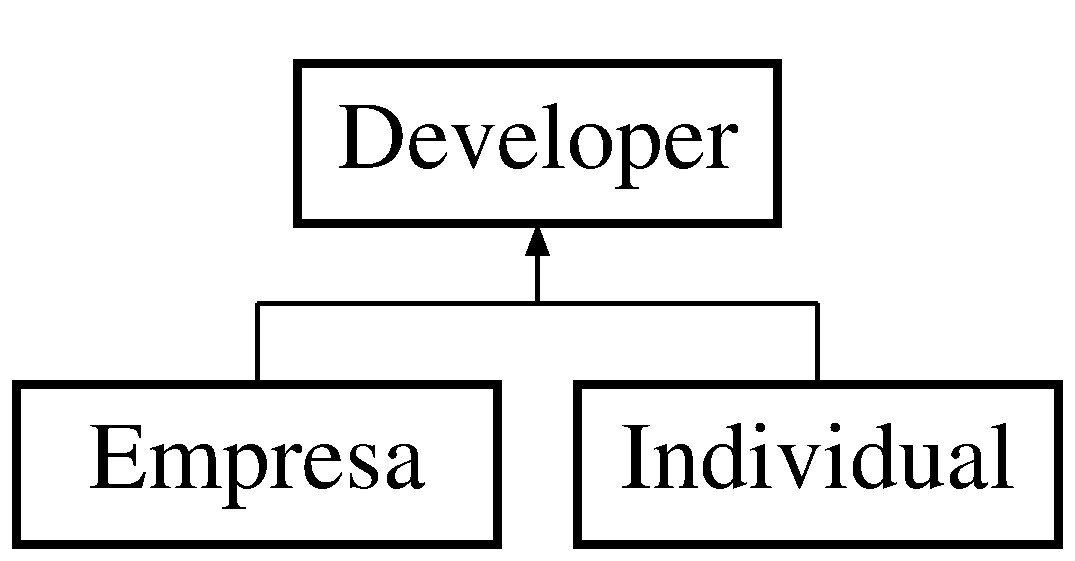
\includegraphics[height=2.000000cm]{class_developer}
\end{center}
\end{figure}
\subsection*{Public Member Functions}
\begin{DoxyCompactItemize}
\item 
\hypertarget{class_developer_abc9b3e48c4a74a074a9a236a58cd76d4}{{\bfseries Developer} (string nome, string id\+\_\+pass)}\label{class_developer_abc9b3e48c4a74a074a9a236a58cd76d4}

\item 
\hypertarget{class_developer_a6db6c9b58043644f773bd39cf8d0207a}{{\bfseries Developer} (int id, string nome, double saldo, string id\+\_\+pass)}\label{class_developer_a6db6c9b58043644f773bd39cf8d0207a}

\item 
\hypertarget{class_developer_a45a0742f3889353f6d17f1f92cb9060f}{string {\bfseries get\+Nome} () const }\label{class_developer_a45a0742f3889353f6d17f1f92cb9060f}

\item 
\hypertarget{class_developer_a81f51af18ee657401e680deb1fe9f38b}{double {\bfseries get\+Saldo} () const }\label{class_developer_a81f51af18ee657401e680deb1fe9f38b}

\item 
\hypertarget{class_developer_a6d56d8bd26ad1df91a2b29ce87e504e4}{void {\bfseries set\+Saldo} (unsigned int s)}\label{class_developer_a6d56d8bd26ad1df91a2b29ce87e504e4}

\item 
\hypertarget{class_developer_aeb475466479de236692d58dfde6ac191}{virtual string {\bfseries get\+Type} () const =0}\label{class_developer_aeb475466479de236692d58dfde6ac191}

\item 
\hypertarget{class_developer_a38d348d3bb05d3505222bee95c29b2f5}{virtual string {\bfseries get\+Extra} () const =0}\label{class_developer_a38d348d3bb05d3505222bee95c29b2f5}

\item 
\hypertarget{class_developer_affa6ed0c90caf781a20d6fb32940f092}{virtual void {\bfseries set\+Extra} (string info)=0}\label{class_developer_affa6ed0c90caf781a20d6fb32940f092}

\item 
\hypertarget{class_developer_a62488b1ca4ddd82fc0797d3de0123bde}{int {\bfseries get\+Id} () const }\label{class_developer_a62488b1ca4ddd82fc0797d3de0123bde}

\item 
\hypertarget{class_developer_aa84da30abf0b1db518d62825f407c520}{void {\bfseries set\+Id} (int id)}\label{class_developer_aa84da30abf0b1db518d62825f407c520}

\item 
\hypertarget{class_developer_a8e5fdafcd4f78c1ea913e2dc09086caa}{string {\bfseries get\+Id\+Pass} () const }\label{class_developer_a8e5fdafcd4f78c1ea913e2dc09086caa}

\item 
\hypertarget{class_developer_a89801e2863c0548f539beb3077e4f6fc}{unsigned int {\bfseries get\+Next\+Id} () const }\label{class_developer_a89801e2863c0548f539beb3077e4f6fc}

\end{DoxyCompactItemize}
\subsection*{Static Public Member Functions}
\begin{DoxyCompactItemize}
\item 
\hypertarget{class_developer_abc49de08222dae89d042daeff3ad8098}{static void {\bfseries set\+Next\+I\+D} (unsigned int i)}\label{class_developer_abc49de08222dae89d042daeff3ad8098}

\end{DoxyCompactItemize}
\subsection*{Protected Attributes}
\begin{DoxyCompactItemize}
\item 
\hypertarget{class_developer_a4e09440e28b980b66fe81402b5878332}{int {\bfseries id}}\label{class_developer_a4e09440e28b980b66fe81402b5878332}

\item 
\hypertarget{class_developer_ac93712aacdeeed34b0d5ea3723be8639}{string {\bfseries nome}}\label{class_developer_ac93712aacdeeed34b0d5ea3723be8639}

\item 
\hypertarget{class_developer_a87c8d2a8bec77c561d29a82d93d34d40}{double {\bfseries saldo} =0}\label{class_developer_a87c8d2a8bec77c561d29a82d93d34d40}

\item 
\hypertarget{class_developer_a2747bee58df1c3c0a74a7932d1cb8d3e}{string {\bfseries id\+\_\+pass}}\label{class_developer_a2747bee58df1c3c0a74a7932d1cb8d3e}

\end{DoxyCompactItemize}
\subsection*{Static Protected Attributes}
\begin{DoxyCompactItemize}
\item 
\hypertarget{class_developer_a54dcfbe646de46842a473b19ff56a3fd}{static unsigned int {\bfseries next\+\_\+id} = 1}\label{class_developer_a54dcfbe646de46842a473b19ff56a3fd}

\end{DoxyCompactItemize}


The documentation for this class was generated from the following files\+:\begin{DoxyCompactItemize}
\item 
src/Developer.\+h\item 
src/Developer.\+cpp\end{DoxyCompactItemize}

\hypertarget{class_empresa}{\section{Empresa Class Reference}
\label{class_empresa}\index{Empresa@{Empresa}}
}
Inheritance diagram for Empresa\+:\begin{figure}[H]
\begin{center}
\leavevmode
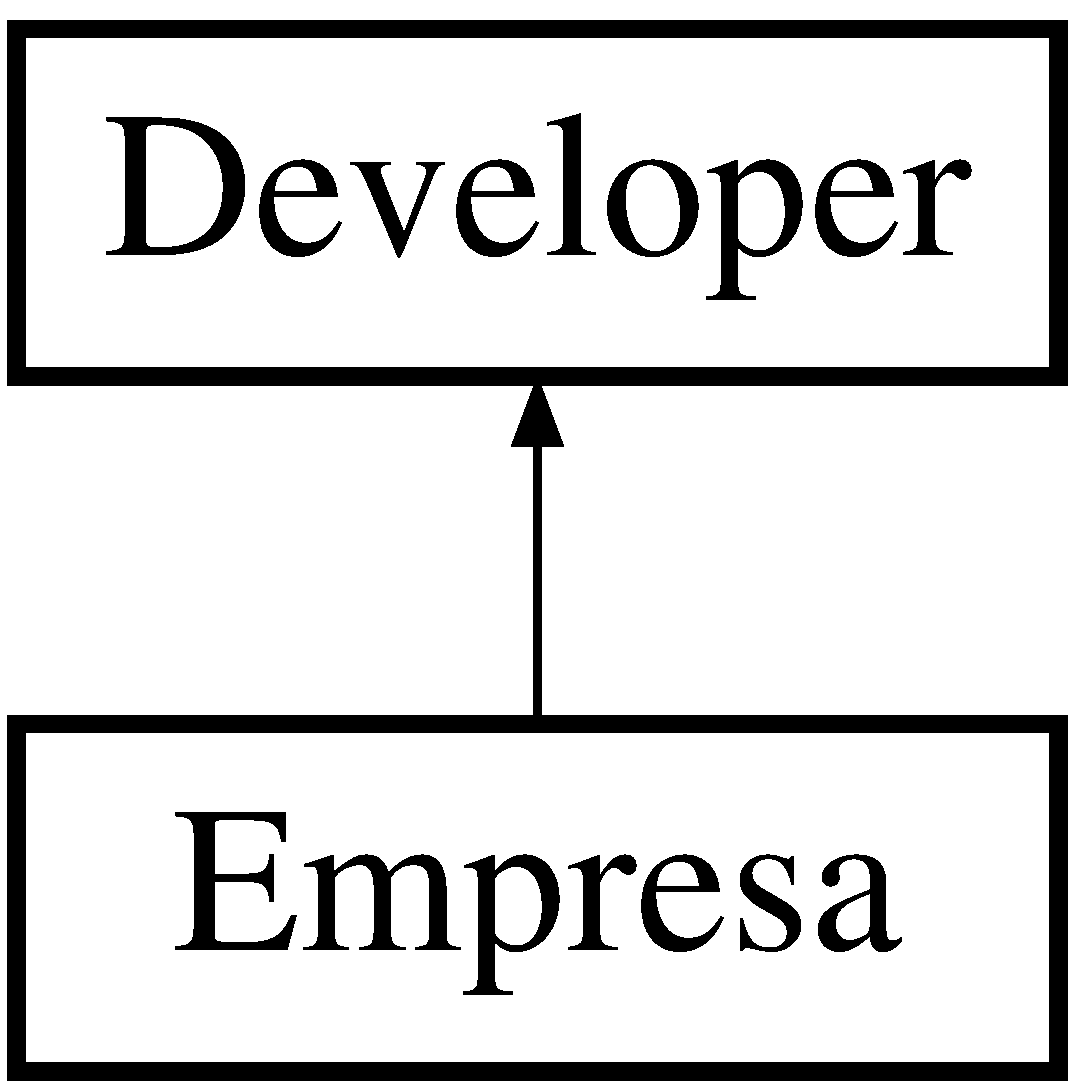
\includegraphics[height=2.000000cm]{class_empresa}
\end{center}
\end{figure}
\subsection*{Public Member Functions}
\begin{DoxyCompactItemize}
\item 
\hypertarget{class_empresa_a340762d9313904da4b41b722ea63935e}{{\bfseries Empresa} (string nome, string id\+\_\+pass, string N\+I\+F)}\label{class_empresa_a340762d9313904da4b41b722ea63935e}

\item 
\hypertarget{class_empresa_acc6cc9b9831e31ede97e4505e0446280}{{\bfseries Empresa} (int id, string nome, double saldo, string id\+\_\+pass, string N\+I\+F)}\label{class_empresa_acc6cc9b9831e31ede97e4505e0446280}

\item 
\hypertarget{class_empresa_ac0c678ba135778e8c62ba4944a68e925}{string {\bfseries get\+Extra} () const }\label{class_empresa_ac0c678ba135778e8c62ba4944a68e925}

\item 
\hypertarget{class_empresa_a85c63a96090672cbc2a572865ec20f44}{string {\bfseries get\+Type} () const }\label{class_empresa_a85c63a96090672cbc2a572865ec20f44}

\item 
\hypertarget{class_empresa_ad6923e466ff3289e0bfb2e777ef41ee9}{void {\bfseries set\+Extra} (string info)}\label{class_empresa_ad6923e466ff3289e0bfb2e777ef41ee9}

\end{DoxyCompactItemize}
\subsection*{Additional Inherited Members}


The documentation for this class was generated from the following files\+:\begin{DoxyCompactItemize}
\item 
src/Developer.\+h\item 
src/Developer.\+cpp\end{DoxyCompactItemize}

\hypertarget{class_file___exp}{\section{File\+\_\+\+Exp Class Reference}
\label{class_file___exp}\index{File\+\_\+\+Exp@{File\+\_\+\+Exp}}
}


Classe para ajudar no tratamento de excepcoes relacionada com os ficheiros.  




{\ttfamily \#include $<$App\+Store.\+h$>$}

\subsection*{Public Member Functions}
\begin{DoxyCompactItemize}
\item 
\hyperlink{class_file___exp_a58f6ca21d2f005ac65bfd05dce33d5c3}{File\+\_\+\+Exp} (unsigned int id, string descricao)
\item 
string \hyperlink{class_file___exp_a8c54a476c0b327bc50071d53bb1326e8}{get\+Descricao\+Erro} () const 
\item 
void \hyperlink{class_file___exp_a0b9435b9ae23d16e1e9041d493f4cd12}{set\+Descricao\+Erro} (string descricao\+Erro)
\item 
unsigned int \hyperlink{class_file___exp_a12f0d708ab52cf35bba854edc1c8b4ce}{get\+Id\+Erro} () const 
\item 
void \hyperlink{class_file___exp_a05c75e2239f556dfed4818575cd010c7}{set\+Id\+Erro} (unsigned int id\+Erro)
\end{DoxyCompactItemize}


\subsection{Detailed Description}
Classe para ajudar no tratamento de excepcoes relacionada com os ficheiros. 

\subsection{Constructor \& Destructor Documentation}
\hypertarget{class_file___exp_a58f6ca21d2f005ac65bfd05dce33d5c3}{\index{File\+\_\+\+Exp@{File\+\_\+\+Exp}!File\+\_\+\+Exp@{File\+\_\+\+Exp}}
\index{File\+\_\+\+Exp@{File\+\_\+\+Exp}!File\+\_\+\+Exp@{File\+\_\+\+Exp}}
\subsubsection[{File\+\_\+\+Exp}]{\setlength{\rightskip}{0pt plus 5cm}File\+\_\+\+Exp\+::\+File\+\_\+\+Exp (
\begin{DoxyParamCaption}
\item[{unsigned int}]{id, }
\item[{string}]{descricao}
\end{DoxyParamCaption}
)}}\label{class_file___exp_a58f6ca21d2f005ac65bfd05dce33d5c3}
Construtor para Excepcao do Ficheiro 
\begin{DoxyParams}{Parameters}
{\em id} & Id Erro \\
\hline
{\em descricao} & D\+Escricao Erro \\
\hline
\end{DoxyParams}


\subsection{Member Function Documentation}
\hypertarget{class_file___exp_a8c54a476c0b327bc50071d53bb1326e8}{\index{File\+\_\+\+Exp@{File\+\_\+\+Exp}!get\+Descricao\+Erro@{get\+Descricao\+Erro}}
\index{get\+Descricao\+Erro@{get\+Descricao\+Erro}!File\+\_\+\+Exp@{File\+\_\+\+Exp}}
\subsubsection[{get\+Descricao\+Erro}]{\setlength{\rightskip}{0pt plus 5cm}string File\+\_\+\+Exp\+::get\+Descricao\+Erro (
\begin{DoxyParamCaption}
{}
\end{DoxyParamCaption}
) const}}\label{class_file___exp_a8c54a476c0b327bc50071d53bb1326e8}
Getter Descricao Erro \begin{DoxyReturn}{Returns}
String Descricao 
\end{DoxyReturn}
\hypertarget{class_file___exp_a12f0d708ab52cf35bba854edc1c8b4ce}{\index{File\+\_\+\+Exp@{File\+\_\+\+Exp}!get\+Id\+Erro@{get\+Id\+Erro}}
\index{get\+Id\+Erro@{get\+Id\+Erro}!File\+\_\+\+Exp@{File\+\_\+\+Exp}}
\subsubsection[{get\+Id\+Erro}]{\setlength{\rightskip}{0pt plus 5cm}unsigned int File\+\_\+\+Exp\+::get\+Id\+Erro (
\begin{DoxyParamCaption}
{}
\end{DoxyParamCaption}
) const}}\label{class_file___exp_a12f0d708ab52cf35bba854edc1c8b4ce}
Getter do Id Erro \begin{DoxyReturn}{Returns}
Int Id Erro 
\end{DoxyReturn}
\hypertarget{class_file___exp_a0b9435b9ae23d16e1e9041d493f4cd12}{\index{File\+\_\+\+Exp@{File\+\_\+\+Exp}!set\+Descricao\+Erro@{set\+Descricao\+Erro}}
\index{set\+Descricao\+Erro@{set\+Descricao\+Erro}!File\+\_\+\+Exp@{File\+\_\+\+Exp}}
\subsubsection[{set\+Descricao\+Erro}]{\setlength{\rightskip}{0pt plus 5cm}void File\+\_\+\+Exp\+::set\+Descricao\+Erro (
\begin{DoxyParamCaption}
\item[{string}]{descricao\+Erro}
\end{DoxyParamCaption}
)}}\label{class_file___exp_a0b9435b9ae23d16e1e9041d493f4cd12}
Setter Descricao Erro 
\begin{DoxyParams}{Parameters}
{\em descricao\+Erro} & Nova Descricao do Erro \\
\hline
\end{DoxyParams}
\hypertarget{class_file___exp_a05c75e2239f556dfed4818575cd010c7}{\index{File\+\_\+\+Exp@{File\+\_\+\+Exp}!set\+Id\+Erro@{set\+Id\+Erro}}
\index{set\+Id\+Erro@{set\+Id\+Erro}!File\+\_\+\+Exp@{File\+\_\+\+Exp}}
\subsubsection[{set\+Id\+Erro}]{\setlength{\rightskip}{0pt plus 5cm}void File\+\_\+\+Exp\+::set\+Id\+Erro (
\begin{DoxyParamCaption}
\item[{unsigned int}]{id\+Erro}
\end{DoxyParamCaption}
)}}\label{class_file___exp_a05c75e2239f556dfed4818575cd010c7}
Getter Id Erro 
\begin{DoxyParams}{Parameters}
{\em id\+Erro} & Novo Id para o Erro \\
\hline
\end{DoxyParams}


The documentation for this class was generated from the following files\+:\begin{DoxyCompactItemize}
\item 
src/App\+Store.\+h\item 
src/App\+Store.\+cpp\end{DoxyCompactItemize}

\hypertarget{class_individual}{\section{Individual Class Reference}
\label{class_individual}\index{Individual@{Individual}}
}
Inheritance diagram for Individual\+:\begin{figure}[H]
\begin{center}
\leavevmode
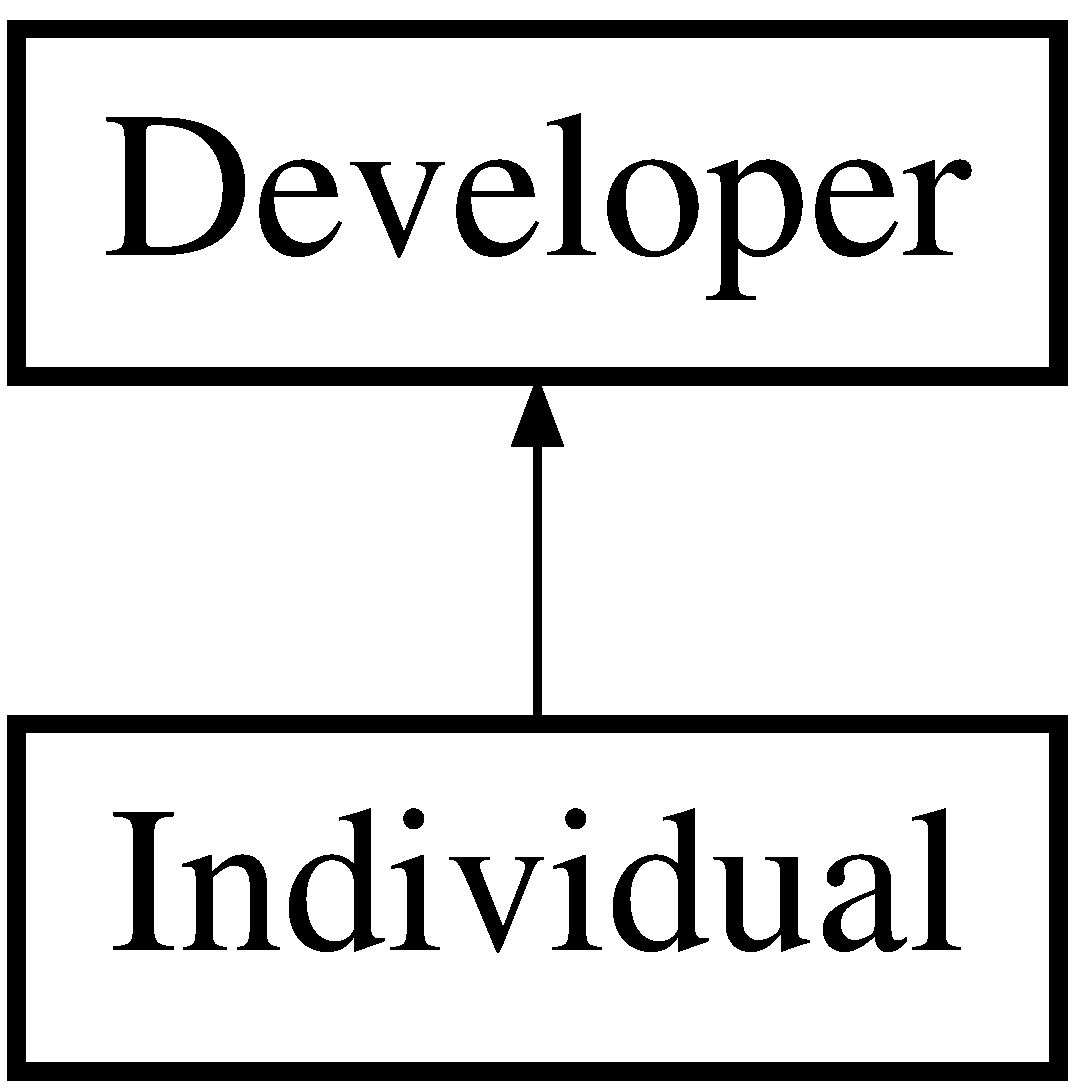
\includegraphics[height=2.000000cm]{class_individual}
\end{center}
\end{figure}
\subsection*{Public Member Functions}
\begin{DoxyCompactItemize}
\item 
\hypertarget{class_individual_abb6c669a8218f6fc95d985f2219c7d2b}{{\bfseries Individual} (string nome, string id\+\_\+pass, string morada, string Nome\+Pessoal)}\label{class_individual_abb6c669a8218f6fc95d985f2219c7d2b}

\item 
\hypertarget{class_individual_adfda751f854c8687761fdd8f803096b2}{{\bfseries Individual} (int id, string nome, double saldo, string id\+\_\+pass, string morada, string Nome\+Pessoal)}\label{class_individual_adfda751f854c8687761fdd8f803096b2}

\item 
\hypertarget{class_individual_ace4ce273559198ae0e57ec1b93381eba}{string {\bfseries get\+Extra} () const }\label{class_individual_ace4ce273559198ae0e57ec1b93381eba}

\item 
\hypertarget{class_individual_a85830ece8fc5dcce9ae340d0d2f931f5}{void {\bfseries set\+Extra} (string info)}\label{class_individual_a85830ece8fc5dcce9ae340d0d2f931f5}

\item 
\hypertarget{class_individual_a3bcf8404908f826e5408a0ced5fceaac}{bool {\bfseries set\+N\+I\+F} (string nif)}\label{class_individual_a3bcf8404908f826e5408a0ced5fceaac}

\item 
\hypertarget{class_individual_a48b52345ec7fa4d62a2f2fbff5b871bf}{string {\bfseries get\+N\+I\+F} () const }\label{class_individual_a48b52345ec7fa4d62a2f2fbff5b871bf}

\item 
\hypertarget{class_individual_a4d909b32b36b7d6be19f222120a8ee22}{string {\bfseries get\+Morada} () const }\label{class_individual_a4d909b32b36b7d6be19f222120a8ee22}

\item 
\hypertarget{class_individual_afce84244dd6f49434d838a9264948ffb}{bool {\bfseries set\+Morada} (string morada)}\label{class_individual_afce84244dd6f49434d838a9264948ffb}

\item 
\hypertarget{class_individual_ae2705598212cf7aafb460b9a49d858cd}{bool {\bfseries is\+Empresa} ()}\label{class_individual_ae2705598212cf7aafb460b9a49d858cd}

\end{DoxyCompactItemize}
\subsection*{Additional Inherited Members}


The documentation for this class was generated from the following files\+:\begin{DoxyCompactItemize}
\item 
src/Developer.\+h\item 
src/Developer.\+cpp\end{DoxyCompactItemize}

\hypertarget{class_vendas}{\section{Vendas Class Reference}
\label{class_vendas}\index{Vendas@{Vendas}}
}
\subsection*{Public Member Functions}
\begin{DoxyCompactItemize}
\item 
\hypertarget{class_vendas_a82262941ae2af8e2527d1859ebc7f5cd}{{\bfseries Vendas} (float preco, \hyperlink{class_date}{Date} data\+\_\+venda)}\label{class_vendas_a82262941ae2af8e2527d1859ebc7f5cd}

\item 
\hypertarget{class_vendas_a84f1ab71befc84a221bc4961f11cb934}{{\bfseries Vendas} (int id, float preco, \hyperlink{class_date}{Date} data\+\_\+venda, bool retorno, string reclamacao)}\label{class_vendas_a84f1ab71befc84a221bc4961f11cb934}

\item 
\hypertarget{class_vendas_a7e36a98494bec3b57d90afa0536a1be5}{int {\bfseries get\+Id} () const }\label{class_vendas_a7e36a98494bec3b57d90afa0536a1be5}

\item 
\hypertarget{class_vendas_aa5c8bcaced98ded9a22444ddf5935566}{float {\bfseries get\+Preco} () const }\label{class_vendas_aa5c8bcaced98ded9a22444ddf5935566}

\item 
\hypertarget{class_vendas_ab4f3bd058d7cfe6fc837e7804b9b3dcf}{\hyperlink{class_date}{Date} {\bfseries get\+Data} () const }\label{class_vendas_ab4f3bd058d7cfe6fc837e7804b9b3dcf}

\item 
\hypertarget{class_vendas_ab900328b9ac3c5e072ad6d7a42f530a3}{\hyperlink{class_app}{App} $\ast$ {\bfseries get\+App} () const }\label{class_vendas_ab900328b9ac3c5e072ad6d7a42f530a3}

\item 
\hypertarget{class_vendas_aeb3fa665d5c3aaf74caf7c1f024f545c}{void {\bfseries set\+App} (\hyperlink{class_app}{App} $\ast$app)}\label{class_vendas_aeb3fa665d5c3aaf74caf7c1f024f545c}

\item 
\hypertarget{class_vendas_a558102d2f9a43bd42bffcdbdd5289555}{\hyperlink{class_date}{Date} {\bfseries get\+Data\+Venda} () const }\label{class_vendas_a558102d2f9a43bd42bffcdbdd5289555}

\item 
\hypertarget{class_vendas_a3a23da44b124f50b3e73e5f568046695}{unsigned int {\bfseries get\+Next\+Id} () const }\label{class_vendas_a3a23da44b124f50b3e73e5f568046695}

\item 
\hypertarget{class_vendas_a13064baa0f6c550cd433946c96a6d0aa}{string {\bfseries get\+Reclamacao} () const }\label{class_vendas_a13064baa0f6c550cd433946c96a6d0aa}

\item 
\hypertarget{class_vendas_a1f5542e8c66cbe9114a7968ffd10d5e2}{bool {\bfseries is\+Retorno} () const }\label{class_vendas_a1f5542e8c66cbe9114a7968ffd10d5e2}

\item 
\hypertarget{class_vendas_ac5bf776bb0b33835e5a3d8728db851fc}{void {\bfseries reclamar} (string reclamacao)}\label{class_vendas_ac5bf776bb0b33835e5a3d8728db851fc}

\end{DoxyCompactItemize}
\subsection*{Static Public Member Functions}
\begin{DoxyCompactItemize}
\item 
\hypertarget{class_vendas_a6b007d0524e51c0a48796a6d9fb9948e}{static void {\bfseries set\+Next\+Id} (unsigned int next\+Id)}\label{class_vendas_a6b007d0524e51c0a48796a6d9fb9948e}

\end{DoxyCompactItemize}


The documentation for this class was generated from the following files\+:\begin{DoxyCompactItemize}
\item 
src/Vendas.\+h\item 
src/Vendas.\+cpp\end{DoxyCompactItemize}

\chapter{File Documentation}
\hypertarget{menu_8h}{\section{src/menu.h File Reference}
\label{menu_8h}\index{src/menu.\+h@{src/menu.\+h}}
}
{\ttfamily \#include \char`\"{}App\+Store.\+h\char`\"{}}\\*
{\ttfamily \#include \char`\"{}Cliente.\+h\char`\"{}}\\*
{\ttfamily \#include \char`\"{}App.\+h\char`\"{}}\\*
\subsection*{Macros}
\begin{DoxyCompactItemize}
\item 
\#define \hyperlink{menu_8h_a7b3b25cba33b07c303f3060fe41887f6}{B\+L\+A\+C\+K}~0
\item 
\hypertarget{menu_8h_a79d10e672abb49ad63eeaa8aaef57c38}{\#define {\bfseries B\+L\+U\+E}~1}\label{menu_8h_a79d10e672abb49ad63eeaa8aaef57c38}

\item 
\hypertarget{menu_8h_acfbc006ea433ad708fdee3e82996e721}{\#define {\bfseries G\+R\+E\+E\+N}~2}\label{menu_8h_acfbc006ea433ad708fdee3e82996e721}

\item 
\hypertarget{menu_8h_a03f3dfd90aa5fafc6c690f215b489976}{\#define {\bfseries A\+Q\+U\+A}~3}\label{menu_8h_a03f3dfd90aa5fafc6c690f215b489976}

\item 
\hypertarget{menu_8h_a8d23feea868a983c8c2b661e1e16972f}{\#define {\bfseries R\+E\+D}~4}\label{menu_8h_a8d23feea868a983c8c2b661e1e16972f}

\item 
\hypertarget{menu_8h_a0bb0b009e7a7390473ace4d98bd843c0}{\#define {\bfseries P\+U\+R\+P\+L\+E}~5}\label{menu_8h_a0bb0b009e7a7390473ace4d98bd843c0}

\item 
\hypertarget{menu_8h_abf681265909adf3d3e8116c93c0ba179}{\#define {\bfseries Y\+E\+L\+L\+O\+W}~6}\label{menu_8h_abf681265909adf3d3e8116c93c0ba179}

\item 
\hypertarget{menu_8h_a87b537f5fa5c109d3c05c13d6b18f382}{\#define {\bfseries W\+H\+I\+T\+E}~7}\label{menu_8h_a87b537f5fa5c109d3c05c13d6b18f382}

\item 
\hypertarget{menu_8h_ae5f70677050eecd8909e0248e07b9e73}{\#define {\bfseries G\+R\+A\+Y}~8}\label{menu_8h_ae5f70677050eecd8909e0248e07b9e73}

\item 
\hypertarget{menu_8h_a5a7142ee95ebc63218ed3aac2ae06b13}{\#define {\bfseries L\+I\+G\+H\+T\+\_\+\+G\+R\+E\+E\+N}~10}\label{menu_8h_a5a7142ee95ebc63218ed3aac2ae06b13}

\item 
\hypertarget{menu_8h_a664c8f5b9d90f79a49a16960b9ccedba}{\#define {\bfseries L\+I\+G\+H\+T\+\_\+\+R\+E\+D}~12}\label{menu_8h_a664c8f5b9d90f79a49a16960b9ccedba}

\end{DoxyCompactItemize}
\subsection*{Functions}
\begin{DoxyCompactItemize}
\item 
void \hyperlink{menu_8h_a163cc3dfe07ad8da53c2a165f796992f}{gotoxy} (int xpos, int ypos)
\item 
void \hyperlink{menu_8h_af6b0777f5781e2a3717af06392d87340}{por\+Data\+No\+Canto} (int xpos, int ypos)
\item 
vector$<$ string $>$ \hyperlink{menu_8h_a8dcf1d43c378c94f999008cd5c141435}{get\+App\+Names} (vector$<$ \hyperlink{class_app}{App} $>$ apps)
\item 
vector$<$ string $>$ \hyperlink{menu_8h_a8e0ba3eb72492e0112a2a9bd94cb0222}{get\+App\+Comentarios} (vector$<$ \hyperlink{class_comentario}{Comentario} $>$ comentarios)
\item 
vector$<$ string $>$ \hyperlink{menu_8h_aca5917a5c99cc4e06191f572ddd6940c}{get\+Dev\+Names} (vector$<$ \hyperlink{class_developer}{Developer} $\ast$ $>$ devs)
\item 
{\footnotesize template$<$typename T $>$ }\\bool \hyperlink{menu_8h_a4e766533a44b1805cdecd69c1504d70a}{verifica\+Pass} (T $\ast$dev\+\_\+or\+\_\+cli)
\item 
void \hyperlink{menu_8h_ad93452507cca9950d9a502c113b07ee6}{print\+Menu\+Scroll} (vector$<$ string $>$ options, int selected\+\_\+option, const unsigned int max\+\_\+per\+\_\+screen)
\item 
void \hyperlink{menu_8h_af40cdeed8b371e9f442b720ef3bd5a85}{cor} (int background, int foreground)
\item 
int \hyperlink{menu_8h_a0bab7caef4d2b37f8cf45547ea4ac6d3}{teclas} ()
\item 
int \hyperlink{menu_8h_a78a4b27d54981f15df0070252b875578}{Restringe\+Opcao\+Teclas} (int min, int max, int opcao)
\item 
void \hyperlink{menu_8h_ac53da549dfcc7985f41132e6220ae565}{menu\+Inicial} (\hyperlink{class_app_store}{App\+Store} \&mieic)
\item 
void \hyperlink{menu_8h_a6191f3f2bea8b377d47e5f425edd84da}{menu\+Login} (\hyperlink{class_app_store}{App\+Store} \&mieic)
\item 
void \hyperlink{menu_8h_a32913b40569bc244121e2fba973d0e34}{menu\+Registar} (\hyperlink{class_app_store}{App\+Store} \&mieic)
\item 
void \hyperlink{menu_8h_a6634ea47c37ac3dad44365df34978a25}{menu\+Login\+Cliente} (\hyperlink{class_app_store}{App\+Store} \&mieic)
\item 
void \hyperlink{menu_8h_af711ceff470d212eb0e42e74981d4910}{menu\+Login\+Developer} (\hyperlink{class_app_store}{App\+Store} \&mieic)
\item 
void \hyperlink{menu_8h_a07cac00b36f9d1591a805b36d2b1fd2e}{menu\+Registar\+Cliente} (\hyperlink{class_app_store}{App\+Store} \&mieic)
\item 
void \hyperlink{menu_8h_ade6e07059d5094c5df4a6d3e7ed225fc}{menu\+Registar\+Developer\+Individual} (\hyperlink{class_app_store}{App\+Store} \&mieic)
\item 
void \hyperlink{menu_8h_a44bc0be430bd5f401d3339d06393a14d}{menu\+Registar\+Developer\+Empresa} (\hyperlink{class_app_store}{App\+Store} \&mieic)
\item 
void \hyperlink{menu_8h_a6eefaa9b64e448d7c89a132f574be79b}{menu\+Cliente} (\hyperlink{class_app_store}{App\+Store} \&mieic)
\item 
void \hyperlink{menu_8h_a34b8329a4e9199ecd8b5a86bf2e4e840}{menu\+Developer} (\hyperlink{class_app_store}{App\+Store} \&mieic)
\item 
void \hyperlink{menu_8h_a4f8b48676f23b8a6a7eab5749a39e705}{menu\+Cliente\+Transacoes} (\hyperlink{class_app_store}{App\+Store} \&mieic)
\item 
void \hyperlink{menu_8h_a6b4091b77e0162f06bf3cc6bf059d7db}{menu\+Cliente\+Definicoes} (\hyperlink{class_app_store}{App\+Store} \&mieic)
\item 
void \hyperlink{menu_8h_a8d542427216a8099353345978cea27a8}{menu\+Developer\+Definicoes} (\hyperlink{class_app_store}{App\+Store} \&mieic)
\item 
void \hyperlink{menu_8h_a34595cb1cba7dc4ac01b86b60b098ecb}{menu\+Developer\+Gerir\+Apps} (\hyperlink{class_app_store}{App\+Store} \&mieic)
\item 
void \hyperlink{menu_8h_ad4d9303c0fa637834ad459c3927c258a}{menu\+Cliente\+Add\+Credito} (\hyperlink{class_app_store}{App\+Store} \&mieic)
\item 
void \hyperlink{menu_8h_acf2f19f77e60bd41485a889def7de4e9}{menu\+Cesto\+Compras} (\hyperlink{class_app_store}{App\+Store} \&mieic)
\item 
void \hyperlink{menu_8h_a13eb1b92f7a3e360e6912a4bf87a478e}{menu\+Historico\+Vendas} (\hyperlink{class_app_store}{App\+Store} \&mieic)
\item 
void \hyperlink{menu_8h_a9a703bf0adece4f3615d4b7f7318f3e6}{menu\+Alterar\+Pass\+Cli} (\hyperlink{class_app_store}{App\+Store} \&mieic)
\item 
void \hyperlink{menu_8h_a41e75906ebfab5d6b6668e588b7482e9}{menu\+Alterar\+Cartao} (\hyperlink{class_app_store}{App\+Store} \&mieic)
\item 
void \hyperlink{menu_8h_ae4192875eb84d8f412857dbba667c11d}{menu\+Apagar\+Conta\+Cli} (\hyperlink{class_app_store}{App\+Store} \&mieic)
\item 
void \hyperlink{menu_8h_a46c31f5ab7c7ef6e8392eb1ed60dd572}{menu\+Alterar\+Pass\+Dev} (\hyperlink{class_app_store}{App\+Store} \&mieic)
\item 
void \hyperlink{menu_8h_a094e1694274f538534152c4029a111a2}{menu\+Alterar\+Morada} (\hyperlink{class_app_store}{App\+Store} \&mieic)
\item 
void \hyperlink{menu_8h_a4663e45c731164bfd236c776d6c83ba4}{menu\+Alterar\+N\+I\+F} (\hyperlink{class_app_store}{App\+Store} \&mieic)
\item 
void \hyperlink{menu_8h_aff77e85990bd91593b140da7bd2b189b}{menu\+Apagar\+Conta\+Dev} (\hyperlink{class_app_store}{App\+Store} \&mieic)
\item 
void \hyperlink{menu_8h_a97cac7505f5894287084209eda3b57c5}{menu\+Ver\+Dev} (\hyperlink{class_app_store}{App\+Store} \&mieic)
\item 
void \hyperlink{menu_8h_a694be05d1f3883cb7e58c124364b8b56}{menu\+Ver\+Cli} (\hyperlink{class_app_store}{App\+Store} \&mieic)
\item 
void \hyperlink{menu_8h_a9619e88ec268f60430d38d1b9f8f35fe}{menu\+Criar\+App} (\hyperlink{class_app_store}{App\+Store} \&mieic)
\item 
void \hyperlink{menu_8h_a57b94e5b624d8873fe39f28f38af97d5}{menu\+Remover\+App} (\hyperlink{class_app_store}{App\+Store} \&mieic)
\item 
void \hyperlink{menu_8h_abc43525e7b000d923858fc38be3cf53c}{menu\+Modificar\+App} (\hyperlink{class_app_store}{App\+Store} \&mieic)
\item 
void \hyperlink{menu_8h_ae9c0826bafa32eb1c832fd954c057693}{menu\+Tira\+Apps\+Cesto} (\hyperlink{class_app_store}{App\+Store} \&mieic)
\item 
void \hyperlink{menu_8h_aa80fc17d3828f5c38f9547cfd08b785a}{menu\+Checkout\+Apps} (\hyperlink{class_app_store}{App\+Store} \&mieic)
\item 
void \hyperlink{menu_8h_a33c0f58b77edd51d4433290358b53f53}{apaga\+Apps\+Nao\+Existentes} (\hyperlink{class_app_store}{App\+Store} \&mieic, \hyperlink{class_cliente}{Cliente} $\ast$cli)
\item 
void \hyperlink{menu_8h_a2cb3e608b54e51094940b1199b2ee037}{menu\+Visita\+Store} (\hyperlink{class_app_store}{App\+Store} \&mieic, unsigned int \&state)
\item 
void \hyperlink{menu_8h_aa7059ce4cdd8d41ac7fea4d69ed8e602}{menu\+Visita\+Store\+Ordenada} (\hyperlink{class_app_store}{App\+Store} \&mieic, unsigned int \&state, vector$<$ \hyperlink{class_app}{App} $>$ apps\+\_\+ordenadas, string tipo\+\_\+ordenacao)
\item 
void \hyperlink{menu_8h_ad3927782add148d5fb6204110050ef3d}{menu\+Lista\+Developer} (\hyperlink{class_app_store}{App\+Store} \&mieic, unsigned int \&state)
\item 
void \hyperlink{menu_8h_ac1fe407808d34bbb9c5bd7651d17e9a7}{menu\+Lista\+Cliente} (\hyperlink{class_app_store}{App\+Store} \&mieic)
\item 
void \hyperlink{menu_8h_ab96196caeb26842aa5db3e6d30cd1641}{menu\+Apps\+Em\+Espera} (\hyperlink{class_app_store}{App\+Store} \&mieic)
\item 
void \hyperlink{menu_8h_a32c3519a225d733f692b9b6e646c2393}{menu\+Remover\+App\+Da\+Store} (\hyperlink{class_app_store}{App\+Store} \&mieic)
\item 
void \hyperlink{menu_8h_aab42f8ce621c3607a899ebebbec31e90}{menu\+Remover\+App\+Fora\+Store\+Perma} (\hyperlink{class_app_store}{App\+Store} \&mieic)
\item 
void \hyperlink{menu_8h_ad2a64115e464068dddee4689ca0f6283}{menu\+Repor\+App\+Store} (\hyperlink{class_app_store}{App\+Store} \&mieic)
\item 
void \hyperlink{menu_8h_ae578034c567d3e6f715bedd93997d30c}{menu\+Modificar\+Apps\+Removidas} (\hyperlink{class_app_store}{App\+Store} \&mieic)
\item 
void \hyperlink{menu_8h_a9ec6435b55f3ec250258fb735c1ccc79}{menu\+Listar\+Apps\+Removidas} (\hyperlink{class_app_store}{App\+Store} \&mieic)
\item 
void \hyperlink{menu_8h_a43e1d3562cb2ea01a65f4eed5d2e000e}{menu\+Modificar\+Apps\+Nao\+Validadas} (\hyperlink{class_app_store}{App\+Store} \&mieic)
\end{DoxyCompactItemize}
\subsection*{Variables}
\begin{DoxyCompactItemize}
\item 
const unsigned int \hyperlink{menu_8h_a7454417415ab1b179bb0a6a707aa4d69}{M\+A\+X\+\_\+\+P\+E\+R\+\_\+\+S\+C\+R\+E\+E\+N} = 6
\item 
const std\+::string \hyperlink{menu_8h_a07b6bc214c08c60cda4376d6a9494275}{A\+D\+M\+I\+N\+\_\+\+P\+A\+S\+S} = \char`\"{}123\char`\"{}
\item 
\hyperlink{class_developer}{Developer} $\ast$ \hyperlink{menu_8h_a2f1da29a33c4776c66ea396c75b634c7}{dev\+\_\+act}
\item 
\hyperlink{class_cliente}{Cliente} $\ast$ \hyperlink{menu_8h_a10cde3b7e2aaa878766a5afb37113065}{cli\+\_\+act}
\end{DoxyCompactItemize}


\subsection{Detailed Description}
Ficheiro com funcoes do menu 

\subsection{Macro Definition Documentation}
\hypertarget{menu_8h_a7b3b25cba33b07c303f3060fe41887f6}{\index{menu.\+h@{menu.\+h}!B\+L\+A\+C\+K@{B\+L\+A\+C\+K}}
\index{B\+L\+A\+C\+K@{B\+L\+A\+C\+K}!menu.\+h@{menu.\+h}}
\subsubsection[{B\+L\+A\+C\+K}]{\setlength{\rightskip}{0pt plus 5cm}\#define B\+L\+A\+C\+K~0}}\label{menu_8h_a7b3b25cba33b07c303f3060fe41887f6}
$<$ Macros de cores para usar no menu 

\subsection{Function Documentation}
\hypertarget{menu_8h_a33c0f58b77edd51d4433290358b53f53}{\index{menu.\+h@{menu.\+h}!apaga\+Apps\+Nao\+Existentes@{apaga\+Apps\+Nao\+Existentes}}
\index{apaga\+Apps\+Nao\+Existentes@{apaga\+Apps\+Nao\+Existentes}!menu.\+h@{menu.\+h}}
\subsubsection[{apaga\+Apps\+Nao\+Existentes}]{\setlength{\rightskip}{0pt plus 5cm}void apaga\+Apps\+Nao\+Existentes (
\begin{DoxyParamCaption}
\item[{{\bf App\+Store} \&}]{mieic, }
\item[{{\bf Cliente} $\ast$}]{cli}
\end{DoxyParamCaption}
)}}\label{menu_8h_a33c0f58b77edd51d4433290358b53f53}
Funcao chamada no cesto de compras, que compara as apps do cesto de compras com as existentes. Se entretanto uma app tiver desaparecido do vetor de apps (por exemplo, se um developer tiver apagado uma app, por exemplo), esta app sera tambem apagada do cesto de compras. 
\begin{DoxyParams}{Parameters}
{\em mieic} & \hyperlink{class_app_store}{App\+Store} criada no main, passada por referencia para poder ser alterada \\
\hline
{\em cli} & Pointer para o cliente atual, a cujo cesto de compras se acede \\
\hline
\end{DoxyParams}
\hypertarget{menu_8h_af40cdeed8b371e9f442b720ef3bd5a85}{\index{menu.\+h@{menu.\+h}!cor@{cor}}
\index{cor@{cor}!menu.\+h@{menu.\+h}}
\subsubsection[{cor}]{\setlength{\rightskip}{0pt plus 5cm}void cor (
\begin{DoxyParamCaption}
\item[{int}]{background, }
\item[{int}]{foreground}
\end{DoxyParamCaption}
)}}\label{menu_8h_af40cdeed8b371e9f442b720ef3bd5a85}
Altera a cor do background e foreground para os valores/cores especificadas 
\begin{DoxyParams}{Parameters}
{\em background} & Cor para o fundo do A\+P\+I -\/ usa-\/se aqui uma das macros definidas \\
\hline
{\em foreground} & Cor para o foreground/letra do A\+P\+I -\/ usa-\/se aqui uma das macros definidas \\
\hline
\end{DoxyParams}
\hypertarget{menu_8h_a8e0ba3eb72492e0112a2a9bd94cb0222}{\index{menu.\+h@{menu.\+h}!get\+App\+Comentarios@{get\+App\+Comentarios}}
\index{get\+App\+Comentarios@{get\+App\+Comentarios}!menu.\+h@{menu.\+h}}
\subsubsection[{get\+App\+Comentarios}]{\setlength{\rightskip}{0pt plus 5cm}vector$<$string$>$ get\+App\+Comentarios (
\begin{DoxyParamCaption}
\item[{vector$<$ {\bf Comentario} $>$}]{comentarios}
\end{DoxyParamCaption}
)}}\label{menu_8h_a8e0ba3eb72492e0112a2a9bd94cb0222}
Pega num vetor de comentarios e forma frases do tipo \char`\"{}\+Cliente x -\/ classificacao -\/ comentario\char`\"{} 
\begin{DoxyParams}{Parameters}
{\em comentarios} & Vetor com objetos do tipo \hyperlink{class_comentario}{Comentario} \\
\hline
\end{DoxyParams}
\begin{DoxyReturn}{Returns}
Devolve o vetor (de strings) com a concatenacao de \hyperlink{class_cliente}{Cliente} -\/ classificacao -\/ comentario 
\end{DoxyReturn}
\hypertarget{menu_8h_a8dcf1d43c378c94f999008cd5c141435}{\index{menu.\+h@{menu.\+h}!get\+App\+Names@{get\+App\+Names}}
\index{get\+App\+Names@{get\+App\+Names}!menu.\+h@{menu.\+h}}
\subsubsection[{get\+App\+Names}]{\setlength{\rightskip}{0pt plus 5cm}vector$<$string$>$ get\+App\+Names (
\begin{DoxyParamCaption}
\item[{vector$<$ {\bf App} $>$}]{apps}
\end{DoxyParamCaption}
)}}\label{menu_8h_a8dcf1d43c378c94f999008cd5c141435}
Pega num vetor de apps e cria um vetor de strings com o nome das apps 
\begin{DoxyParams}{Parameters}
{\em apps} & Vetor com objetos do tipo \hyperlink{class_app}{App} \\
\hline
\end{DoxyParams}
\begin{DoxyReturn}{Returns}
Devolve o vetor (de strings) com os nomes das apps inseridas como argumento 
\end{DoxyReturn}
\hypertarget{menu_8h_aca5917a5c99cc4e06191f572ddd6940c}{\index{menu.\+h@{menu.\+h}!get\+Dev\+Names@{get\+Dev\+Names}}
\index{get\+Dev\+Names@{get\+Dev\+Names}!menu.\+h@{menu.\+h}}
\subsubsection[{get\+Dev\+Names}]{\setlength{\rightskip}{0pt plus 5cm}vector$<$string$>$ get\+Dev\+Names (
\begin{DoxyParamCaption}
\item[{vector$<$ {\bf Developer} $\ast$ $>$}]{devs}
\end{DoxyParamCaption}
)}}\label{menu_8h_aca5917a5c99cc4e06191f572ddd6940c}

\begin{DoxyParams}{Parameters}
{\em devs} & Vetor com objetos do tipo Developer$\ast$ \\
\hline
\end{DoxyParams}
\begin{DoxyReturn}{Returns}
Devolve o vetor (de strings) com os nomes dos developers inseridos como argumento 
\end{DoxyReturn}
\hypertarget{menu_8h_a163cc3dfe07ad8da53c2a165f796992f}{\index{menu.\+h@{menu.\+h}!gotoxy@{gotoxy}}
\index{gotoxy@{gotoxy}!menu.\+h@{menu.\+h}}
\subsubsection[{gotoxy}]{\setlength{\rightskip}{0pt plus 5cm}void gotoxy (
\begin{DoxyParamCaption}
\item[{int}]{xpos, }
\item[{int}]{ypos}
\end{DoxyParamCaption}
)}}\label{menu_8h_a163cc3dfe07ad8da53c2a165f796992f}
Mete o cursor numa posicao do ecra, para se poder escrever nesse local diretamente


\begin{DoxyParams}{Parameters}
{\em xpos} & Coluna para a qual o cursor vai \\
\hline
{\em ypos} & Linha para a qual o cursor vai \\
\hline
\end{DoxyParams}
\hypertarget{menu_8h_a41e75906ebfab5d6b6668e588b7482e9}{\index{menu.\+h@{menu.\+h}!menu\+Alterar\+Cartao@{menu\+Alterar\+Cartao}}
\index{menu\+Alterar\+Cartao@{menu\+Alterar\+Cartao}!menu.\+h@{menu.\+h}}
\subsubsection[{menu\+Alterar\+Cartao}]{\setlength{\rightskip}{0pt plus 5cm}void menu\+Alterar\+Cartao (
\begin{DoxyParamCaption}
\item[{{\bf App\+Store} \&}]{mieic}
\end{DoxyParamCaption}
)}}\label{menu_8h_a41e75906ebfab5d6b6668e588b7482e9}
Menu onde, apos chamar a confirmacao da Password, o cliente pode alterar o seu Nr. Cartao de Credito. Regressa depois ao menu de definicoes de cliente. 
\begin{DoxyParams}{Parameters}
{\em mieic} & \hyperlink{class_app_store}{App\+Store} criada no main, passada por referencia para poder ser alterada \\
\hline
\end{DoxyParams}
\hypertarget{menu_8h_a094e1694274f538534152c4029a111a2}{\index{menu.\+h@{menu.\+h}!menu\+Alterar\+Morada@{menu\+Alterar\+Morada}}
\index{menu\+Alterar\+Morada@{menu\+Alterar\+Morada}!menu.\+h@{menu.\+h}}
\subsubsection[{menu\+Alterar\+Morada}]{\setlength{\rightskip}{0pt plus 5cm}void menu\+Alterar\+Morada (
\begin{DoxyParamCaption}
\item[{{\bf App\+Store} \&}]{mieic}
\end{DoxyParamCaption}
)}}\label{menu_8h_a094e1694274f538534152c4029a111a2}
Menu onde, apos chamar a confirmacao da Password, o developer pode alterar a sua morada Regressa depois ao menu de definicoes do developer 
\begin{DoxyParams}{Parameters}
{\em mieic} & \hyperlink{class_app_store}{App\+Store} criada no main, passada por referencia para poder ser alterada \\
\hline
\end{DoxyParams}
\hypertarget{menu_8h_a4663e45c731164bfd236c776d6c83ba4}{\index{menu.\+h@{menu.\+h}!menu\+Alterar\+N\+I\+F@{menu\+Alterar\+N\+I\+F}}
\index{menu\+Alterar\+N\+I\+F@{menu\+Alterar\+N\+I\+F}!menu.\+h@{menu.\+h}}
\subsubsection[{menu\+Alterar\+N\+I\+F}]{\setlength{\rightskip}{0pt plus 5cm}void menu\+Alterar\+N\+I\+F (
\begin{DoxyParamCaption}
\item[{{\bf App\+Store} \&}]{mieic}
\end{DoxyParamCaption}
)}}\label{menu_8h_a4663e45c731164bfd236c776d6c83ba4}
Menu onde, apos chamar a confirmacao da Password, o developer pode alterar a sua morada Regressa depois ao menu de definicoes do developer 
\begin{DoxyParams}{Parameters}
{\em mieic} & \hyperlink{class_app_store}{App\+Store} criada no main, passada por referencia para poder ser alterada \\
\hline
\end{DoxyParams}
\hypertarget{menu_8h_a9a703bf0adece4f3615d4b7f7318f3e6}{\index{menu.\+h@{menu.\+h}!menu\+Alterar\+Pass\+Cli@{menu\+Alterar\+Pass\+Cli}}
\index{menu\+Alterar\+Pass\+Cli@{menu\+Alterar\+Pass\+Cli}!menu.\+h@{menu.\+h}}
\subsubsection[{menu\+Alterar\+Pass\+Cli}]{\setlength{\rightskip}{0pt plus 5cm}void menu\+Alterar\+Pass\+Cli (
\begin{DoxyParamCaption}
\item[{{\bf App\+Store} \&}]{mieic}
\end{DoxyParamCaption}
)}}\label{menu_8h_a9a703bf0adece4f3615d4b7f7318f3e6}
Menu onde, apos chamar a confirmacao da Password, o cliente pode alterar a sua password. Regressa depois ao menu de definicoes de cliente. 
\begin{DoxyParams}{Parameters}
{\em mieic} & \hyperlink{class_app_store}{App\+Store} criada no main, passada por referencia para poder ser alterada \\
\hline
\end{DoxyParams}
\hypertarget{menu_8h_a46c31f5ab7c7ef6e8392eb1ed60dd572}{\index{menu.\+h@{menu.\+h}!menu\+Alterar\+Pass\+Dev@{menu\+Alterar\+Pass\+Dev}}
\index{menu\+Alterar\+Pass\+Dev@{menu\+Alterar\+Pass\+Dev}!menu.\+h@{menu.\+h}}
\subsubsection[{menu\+Alterar\+Pass\+Dev}]{\setlength{\rightskip}{0pt plus 5cm}void menu\+Alterar\+Pass\+Dev (
\begin{DoxyParamCaption}
\item[{{\bf App\+Store} \&}]{mieic}
\end{DoxyParamCaption}
)}}\label{menu_8h_a46c31f5ab7c7ef6e8392eb1ed60dd572}
Opcao do menu de definicoes de developer onde, apos confirmacao da pass, o developer pode escolher alterar a sua pass ou regressar para o menu de definicoes do developer. 
\begin{DoxyParams}{Parameters}
{\em mieic} & \hyperlink{class_app_store}{App\+Store} criada no main, passada por referencia para poder ser alterada \\
\hline
\end{DoxyParams}
\hypertarget{menu_8h_ae4192875eb84d8f412857dbba667c11d}{\index{menu.\+h@{menu.\+h}!menu\+Apagar\+Conta\+Cli@{menu\+Apagar\+Conta\+Cli}}
\index{menu\+Apagar\+Conta\+Cli@{menu\+Apagar\+Conta\+Cli}!menu.\+h@{menu.\+h}}
\subsubsection[{menu\+Apagar\+Conta\+Cli}]{\setlength{\rightskip}{0pt plus 5cm}void menu\+Apagar\+Conta\+Cli (
\begin{DoxyParamCaption}
\item[{{\bf App\+Store} \&}]{mieic}
\end{DoxyParamCaption}
)}}\label{menu_8h_ae4192875eb84d8f412857dbba667c11d}
Opcao do menu onde, apos confirmacao da pass, o \hyperlink{class_cliente}{Cliente} apaga a conta. Regressa depois ao menu Inicial. 
\begin{DoxyParams}{Parameters}
{\em mieic} & \hyperlink{class_app_store}{App\+Store} criada no main, passada por referencia para poder ser alterada \\
\hline
\end{DoxyParams}
\hypertarget{menu_8h_aff77e85990bd91593b140da7bd2b189b}{\index{menu.\+h@{menu.\+h}!menu\+Apagar\+Conta\+Dev@{menu\+Apagar\+Conta\+Dev}}
\index{menu\+Apagar\+Conta\+Dev@{menu\+Apagar\+Conta\+Dev}!menu.\+h@{menu.\+h}}
\subsubsection[{menu\+Apagar\+Conta\+Dev}]{\setlength{\rightskip}{0pt plus 5cm}void menu\+Apagar\+Conta\+Dev (
\begin{DoxyParamCaption}
\item[{{\bf App\+Store} \&}]{mieic}
\end{DoxyParamCaption}
)}}\label{menu_8h_aff77e85990bd91593b140da7bd2b189b}
Opcao do menu onde, apos confirmacao da pass, o \hyperlink{class_developer}{Developer} apaga a password. Regressa depois ao menu Inicial. 
\begin{DoxyParams}{Parameters}
{\em mieic} & \hyperlink{class_app_store}{App\+Store} criada no main, passada por referencia para poder ser alterada \\
\hline
\end{DoxyParams}
\hypertarget{menu_8h_ab96196caeb26842aa5db3e6d30cd1641}{\index{menu.\+h@{menu.\+h}!menu\+Apps\+Em\+Espera@{menu\+Apps\+Em\+Espera}}
\index{menu\+Apps\+Em\+Espera@{menu\+Apps\+Em\+Espera}!menu.\+h@{menu.\+h}}
\subsubsection[{menu\+Apps\+Em\+Espera}]{\setlength{\rightskip}{0pt plus 5cm}void menu\+Apps\+Em\+Espera (
\begin{DoxyParamCaption}
\item[{{\bf App\+Store} \&}]{mieic}
\end{DoxyParamCaption}
)}}\label{menu_8h_ab96196caeb26842aa5db3e6d30cd1641}
Menu que faz validacao das apps em espera na priority\+\_\+queue A validacao so e efetuada apos o admin inserir os seus dados


\begin{DoxyParams}{Parameters}
{\em mieic} & \hyperlink{class_app_store}{App\+Store} criada no main, passada por referencia para poder ser alterada \\
\hline
\end{DoxyParams}
\hypertarget{menu_8h_acf2f19f77e60bd41485a889def7de4e9}{\index{menu.\+h@{menu.\+h}!menu\+Cesto\+Compras@{menu\+Cesto\+Compras}}
\index{menu\+Cesto\+Compras@{menu\+Cesto\+Compras}!menu.\+h@{menu.\+h}}
\subsubsection[{menu\+Cesto\+Compras}]{\setlength{\rightskip}{0pt plus 5cm}void menu\+Cesto\+Compras (
\begin{DoxyParamCaption}
\item[{{\bf App\+Store} \&}]{mieic}
\end{DoxyParamCaption}
)}}\label{menu_8h_acf2f19f77e60bd41485a889def7de4e9}
Menu do \hyperlink{class_cliente}{Cliente} onde sao exibidos os submenus do cesto de compras\+: Ver cesto/checkout, remover items do cesto e regressao ao menu anterior (menu \hyperlink{class_cliente}{Cliente}) 
\begin{DoxyParams}{Parameters}
{\em mieic} & \hyperlink{class_app_store}{App\+Store} criada no main, passada por referencia para poder ser alterada \\
\hline
\end{DoxyParams}
\hypertarget{menu_8h_aa80fc17d3828f5c38f9547cfd08b785a}{\index{menu.\+h@{menu.\+h}!menu\+Checkout\+Apps@{menu\+Checkout\+Apps}}
\index{menu\+Checkout\+Apps@{menu\+Checkout\+Apps}!menu.\+h@{menu.\+h}}
\subsubsection[{menu\+Checkout\+Apps}]{\setlength{\rightskip}{0pt plus 5cm}void menu\+Checkout\+Apps (
\begin{DoxyParamCaption}
\item[{{\bf App\+Store} \&}]{mieic}
\end{DoxyParamCaption}
)}}\label{menu_8h_aa80fc17d3828f5c38f9547cfd08b785a}
Menu onde sao mostradas as apps do cesto, o seu preco total, o seu preco total se for usado um Voucher e o saldo que o cliente tem disponivel. O cliente pode entao escolher fazer o checkout ou regressar. Ao fazer checkout, se tiver Vouchers, podera fazer uso destes, tendo um desconto. 
\begin{DoxyParams}{Parameters}
{\em mieic} & \hyperlink{class_app_store}{App\+Store} criada no main, passada por referencia para poder ser alterada \\
\hline
\end{DoxyParams}
\hypertarget{menu_8h_a6eefaa9b64e448d7c89a132f574be79b}{\index{menu.\+h@{menu.\+h}!menu\+Cliente@{menu\+Cliente}}
\index{menu\+Cliente@{menu\+Cliente}!menu.\+h@{menu.\+h}}
\subsubsection[{menu\+Cliente}]{\setlength{\rightskip}{0pt plus 5cm}void menu\+Cliente (
\begin{DoxyParamCaption}
\item[{{\bf App\+Store} \&}]{mieic}
\end{DoxyParamCaption}
)}}\label{menu_8h_a6eefaa9b64e448d7c89a132f574be79b}
Menu principal de cliente, onde sao exibidas os submenus\+: visitar appstore, mexer nas transacoes e credito, alterar definicoes, ver os atributos e fazer logout. 
\begin{DoxyParams}{Parameters}
{\em mieic} & \hyperlink{class_app_store}{App\+Store} criada no main, passada por referencia para poder ser alterada \\
\hline
\end{DoxyParams}
\hypertarget{menu_8h_ad4d9303c0fa637834ad459c3927c258a}{\index{menu.\+h@{menu.\+h}!menu\+Cliente\+Add\+Credito@{menu\+Cliente\+Add\+Credito}}
\index{menu\+Cliente\+Add\+Credito@{menu\+Cliente\+Add\+Credito}!menu.\+h@{menu.\+h}}
\subsubsection[{menu\+Cliente\+Add\+Credito}]{\setlength{\rightskip}{0pt plus 5cm}void menu\+Cliente\+Add\+Credito (
\begin{DoxyParamCaption}
\item[{{\bf App\+Store} \&}]{mieic}
\end{DoxyParamCaption}
)}}\label{menu_8h_ad4d9303c0fa637834ad459c3927c258a}
Menu onde, apos verificacao do Nr. de cartao de credito, o \hyperlink{class_cliente}{Cliente} escolhe o credito a adicionar a sua conta, podendo regressar sem adicionar credito. 
\begin{DoxyParams}{Parameters}
{\em mieic} & \hyperlink{class_app_store}{App\+Store} criada no main, passada por referencia para poder ser alterada \\
\hline
\end{DoxyParams}
\hypertarget{menu_8h_a6b4091b77e0162f06bf3cc6bf059d7db}{\index{menu.\+h@{menu.\+h}!menu\+Cliente\+Definicoes@{menu\+Cliente\+Definicoes}}
\index{menu\+Cliente\+Definicoes@{menu\+Cliente\+Definicoes}!menu.\+h@{menu.\+h}}
\subsubsection[{menu\+Cliente\+Definicoes}]{\setlength{\rightskip}{0pt plus 5cm}void menu\+Cliente\+Definicoes (
\begin{DoxyParamCaption}
\item[{{\bf App\+Store} \&}]{mieic}
\end{DoxyParamCaption}
)}}\label{menu_8h_a6b4091b77e0162f06bf3cc6bf059d7db}
Menu do \hyperlink{class_cliente}{Cliente} onde ele pode escolher os submenus de Alterar Password, Alterar Nr. Cartao de Credito, e apagar a sua conta 
\begin{DoxyParams}{Parameters}
{\em mieic} & \hyperlink{class_app_store}{App\+Store} criada no main, passada por referencia para poder ser alterada \\
\hline
\end{DoxyParams}
\hypertarget{menu_8h_a4f8b48676f23b8a6a7eab5749a39e705}{\index{menu.\+h@{menu.\+h}!menu\+Cliente\+Transacoes@{menu\+Cliente\+Transacoes}}
\index{menu\+Cliente\+Transacoes@{menu\+Cliente\+Transacoes}!menu.\+h@{menu.\+h}}
\subsubsection[{menu\+Cliente\+Transacoes}]{\setlength{\rightskip}{0pt plus 5cm}void menu\+Cliente\+Transacoes (
\begin{DoxyParamCaption}
\item[{{\bf App\+Store} \&}]{mieic}
\end{DoxyParamCaption}
)}}\label{menu_8h_a4f8b48676f23b8a6a7eab5749a39e705}
Menu do \hyperlink{class_cliente}{Cliente} onde este pode escolher os submenus de Adicionar Credito, ver o seu cesto de compras, rever o seu historico de vendas/compras ou regressar ao menu anterior. 
\begin{DoxyParams}{Parameters}
{\em mieic} & \hyperlink{class_app_store}{App\+Store} criada no main, passada por referencia para poder ser alterada \\
\hline
\end{DoxyParams}
\hypertarget{menu_8h_a9619e88ec268f60430d38d1b9f8f35fe}{\index{menu.\+h@{menu.\+h}!menu\+Criar\+App@{menu\+Criar\+App}}
\index{menu\+Criar\+App@{menu\+Criar\+App}!menu.\+h@{menu.\+h}}
\subsubsection[{menu\+Criar\+App}]{\setlength{\rightskip}{0pt plus 5cm}void menu\+Criar\+App (
\begin{DoxyParamCaption}
\item[{{\bf App\+Store} \&}]{mieic}
\end{DoxyParamCaption}
)}}\label{menu_8h_a9619e88ec268f60430d38d1b9f8f35fe}
Menu onde o \hyperlink{class_developer}{Developer} pode criar uma app, introduzindo os dados desta. Regressa depois ao menu de gestao de apps 
\begin{DoxyParams}{Parameters}
{\em mieic} & \hyperlink{class_app_store}{App\+Store} criada no main, passada por referencia para poder ser alterada \\
\hline
\end{DoxyParams}
\hypertarget{menu_8h_a34b8329a4e9199ecd8b5a86bf2e4e840}{\index{menu.\+h@{menu.\+h}!menu\+Developer@{menu\+Developer}}
\index{menu\+Developer@{menu\+Developer}!menu.\+h@{menu.\+h}}
\subsubsection[{menu\+Developer}]{\setlength{\rightskip}{0pt plus 5cm}void menu\+Developer (
\begin{DoxyParamCaption}
\item[{{\bf App\+Store} \&}]{mieic}
\end{DoxyParamCaption}
)}}\label{menu_8h_a34b8329a4e9199ecd8b5a86bf2e4e840}
Menu principal de developer, onde sao exibidas os submenus\+: visitar appstore, gestao de apps, alterar definicoes, ver os atributos e fazer logout. 
\begin{DoxyParams}{Parameters}
{\em mieic} & \hyperlink{class_app_store}{App\+Store} criada no main, passada por referencia para poder ser alterada \\
\hline
\end{DoxyParams}
\hypertarget{menu_8h_a8d542427216a8099353345978cea27a8}{\index{menu.\+h@{menu.\+h}!menu\+Developer\+Definicoes@{menu\+Developer\+Definicoes}}
\index{menu\+Developer\+Definicoes@{menu\+Developer\+Definicoes}!menu.\+h@{menu.\+h}}
\subsubsection[{menu\+Developer\+Definicoes}]{\setlength{\rightskip}{0pt plus 5cm}void menu\+Developer\+Definicoes (
\begin{DoxyParamCaption}
\item[{{\bf App\+Store} \&}]{mieic}
\end{DoxyParamCaption}
)}}\label{menu_8h_a8d542427216a8099353345978cea27a8}
Menu do \hyperlink{class_developer}{Developer} onde ele pode escolher os submenus de Alterar Password, Alterar morada e apagar a sua conta 
\begin{DoxyParams}{Parameters}
{\em mieic} & \hyperlink{class_app_store}{App\+Store} criada no main, passada por referencia para poder ser alterada \\
\hline
\end{DoxyParams}
\hypertarget{menu_8h_a34595cb1cba7dc4ac01b86b60b098ecb}{\index{menu.\+h@{menu.\+h}!menu\+Developer\+Gerir\+Apps@{menu\+Developer\+Gerir\+Apps}}
\index{menu\+Developer\+Gerir\+Apps@{menu\+Developer\+Gerir\+Apps}!menu.\+h@{menu.\+h}}
\subsubsection[{menu\+Developer\+Gerir\+Apps}]{\setlength{\rightskip}{0pt plus 5cm}void menu\+Developer\+Gerir\+Apps (
\begin{DoxyParamCaption}
\item[{{\bf App\+Store} \&}]{mieic}
\end{DoxyParamCaption}
)}}\label{menu_8h_a34595cb1cba7dc4ac01b86b60b098ecb}
Menu do \hyperlink{class_developer}{Developer} onde este tem opcoes de gestao de Apps que estao na store. Pode criar uma \hyperlink{class_app}{App}, remover uma app ou entrar no menu para alterar uma app 
\begin{DoxyParams}{Parameters}
{\em mieic} & \hyperlink{class_app_store}{App\+Store} criada no main, passada por referencia para poder ser alterada \\
\hline
\end{DoxyParams}
\hypertarget{menu_8h_a13eb1b92f7a3e360e6912a4bf87a478e}{\index{menu.\+h@{menu.\+h}!menu\+Historico\+Vendas@{menu\+Historico\+Vendas}}
\index{menu\+Historico\+Vendas@{menu\+Historico\+Vendas}!menu.\+h@{menu.\+h}}
\subsubsection[{menu\+Historico\+Vendas}]{\setlength{\rightskip}{0pt plus 5cm}void menu\+Historico\+Vendas (
\begin{DoxyParamCaption}
\item[{{\bf App\+Store} \&}]{mieic}
\end{DoxyParamCaption}
)}}\label{menu_8h_a13eb1b92f7a3e360e6912a4bf87a478e}
Menu onde lista as vendas todas existentes do cliente. Ao carregar Esc regressa ao menu de Transacoes 
\begin{DoxyParams}{Parameters}
{\em mieic} & \hyperlink{class_app_store}{App\+Store} criada no main, passada por referencia para poder ser alterada \\
\hline
\end{DoxyParams}
\hypertarget{menu_8h_ac53da549dfcc7985f41132e6220ae565}{\index{menu.\+h@{menu.\+h}!menu\+Inicial@{menu\+Inicial}}
\index{menu\+Inicial@{menu\+Inicial}!menu.\+h@{menu.\+h}}
\subsubsection[{menu\+Inicial}]{\setlength{\rightskip}{0pt plus 5cm}void menu\+Inicial (
\begin{DoxyParamCaption}
\item[{{\bf App\+Store} \&}]{mieic}
\end{DoxyParamCaption}
)}}\label{menu_8h_ac53da549dfcc7985f41132e6220ae565}
Menu inicial onde sao exibidas opcao de login, registo, visita de appstore ou sair do programa, gravando alteracoes 
\begin{DoxyParams}{Parameters}
{\em mieic} & \hyperlink{class_app_store}{App\+Store} criada no main, passada por referencia para poder ser alterada \\
\hline
\end{DoxyParams}
\hypertarget{menu_8h_ac1fe407808d34bbb9c5bd7651d17e9a7}{\index{menu.\+h@{menu.\+h}!menu\+Lista\+Cliente@{menu\+Lista\+Cliente}}
\index{menu\+Lista\+Cliente@{menu\+Lista\+Cliente}!menu.\+h@{menu.\+h}}
\subsubsection[{menu\+Lista\+Cliente}]{\setlength{\rightskip}{0pt plus 5cm}void menu\+Lista\+Cliente (
\begin{DoxyParamCaption}
\item[{{\bf App\+Store} \&}]{mieic}
\end{DoxyParamCaption}
)}}\label{menu_8h_ac1fe407808d34bbb9c5bd7651d17e9a7}
Menu que faz listagem dos clientes existentes, podendo-\/se ver o nome, idade e sexo 
\begin{DoxyParams}{Parameters}
{\em mieic} & \hyperlink{class_app_store}{App\+Store} criada no main, passada por referencia para poder ser alterada \\
\hline
\end{DoxyParams}
\hypertarget{menu_8h_ad3927782add148d5fb6204110050ef3d}{\index{menu.\+h@{menu.\+h}!menu\+Lista\+Developer@{menu\+Lista\+Developer}}
\index{menu\+Lista\+Developer@{menu\+Lista\+Developer}!menu.\+h@{menu.\+h}}
\subsubsection[{menu\+Lista\+Developer}]{\setlength{\rightskip}{0pt plus 5cm}void menu\+Lista\+Developer (
\begin{DoxyParamCaption}
\item[{{\bf App\+Store} \&}]{mieic, }
\item[{unsigned int \&}]{state}
\end{DoxyParamCaption}
)}}\label{menu_8h_ad3927782add148d5fb6204110050ef3d}
Menu que lista os developers existentes, podendo-\/se escolher o developer e o tipo de listagem. O menu chama depois o menu\+Visita\+Store\+Ordenada(...) e faz display do vetor das apps desse developer, ordenadas da maneira escolhida 
\begin{DoxyParams}{Parameters}
{\em mieic} & \hyperlink{class_app_store}{App\+Store} criada no main, passada por referencia para poder ser alterada \\
\hline
{\em state} & Identifica quem visita a store e o que pode ver\+: 0 se for um guest a visitar, 1 se for um developer e 2 se for um cliente \\
\hline
\end{DoxyParams}
\hypertarget{menu_8h_a9ec6435b55f3ec250258fb735c1ccc79}{\index{menu.\+h@{menu.\+h}!menu\+Listar\+Apps\+Removidas@{menu\+Listar\+Apps\+Removidas}}
\index{menu\+Listar\+Apps\+Removidas@{menu\+Listar\+Apps\+Removidas}!menu.\+h@{menu.\+h}}
\subsubsection[{menu\+Listar\+Apps\+Removidas}]{\setlength{\rightskip}{0pt plus 5cm}void menu\+Listar\+Apps\+Removidas (
\begin{DoxyParamCaption}
\item[{{\bf App\+Store} \&}]{mieic}
\end{DoxyParamCaption}
)}}\label{menu_8h_a9ec6435b55f3ec250258fb735c1ccc79}
Menu que lista Apps removidas 
\begin{DoxyParams}{Parameters}
{\em mieic} & \hyperlink{class_app_store}{App\+Store} criada no main, passada por referencia para poder ser alterada \\
\hline
\end{DoxyParams}
\hypertarget{menu_8h_a6191f3f2bea8b377d47e5f425edd84da}{\index{menu.\+h@{menu.\+h}!menu\+Login@{menu\+Login}}
\index{menu\+Login@{menu\+Login}!menu.\+h@{menu.\+h}}
\subsubsection[{menu\+Login}]{\setlength{\rightskip}{0pt plus 5cm}void menu\+Login (
\begin{DoxyParamCaption}
\item[{{\bf App\+Store} \&}]{mieic}
\end{DoxyParamCaption}
)}}\label{menu_8h_a6191f3f2bea8b377d47e5f425edd84da}
Menu para login, onde o user escolhe qual o tipo de login a efetuar, se de \hyperlink{class_developer}{Developer} ou \hyperlink{class_cliente}{Cliente} 
\begin{DoxyParams}{Parameters}
{\em mieic} & \hyperlink{class_app_store}{App\+Store} criada no main, passada por referencia para poder ser alterada \\
\hline
\end{DoxyParams}
\hypertarget{menu_8h_a6634ea47c37ac3dad44365df34978a25}{\index{menu.\+h@{menu.\+h}!menu\+Login\+Cliente@{menu\+Login\+Cliente}}
\index{menu\+Login\+Cliente@{menu\+Login\+Cliente}!menu.\+h@{menu.\+h}}
\subsubsection[{menu\+Login\+Cliente}]{\setlength{\rightskip}{0pt plus 5cm}void menu\+Login\+Cliente (
\begin{DoxyParamCaption}
\item[{{\bf App\+Store} \&}]{mieic}
\end{DoxyParamCaption}
)}}\label{menu_8h_a6634ea47c37ac3dad44365df34978a25}
Menu para Login do cliente, onde este fornece o seu I\+D e password 
\begin{DoxyParams}{Parameters}
{\em mieic} & \hyperlink{class_app_store}{App\+Store} criada no main, passada por referencia para poder ser alterada \\
\hline
\end{DoxyParams}
\hypertarget{menu_8h_af711ceff470d212eb0e42e74981d4910}{\index{menu.\+h@{menu.\+h}!menu\+Login\+Developer@{menu\+Login\+Developer}}
\index{menu\+Login\+Developer@{menu\+Login\+Developer}!menu.\+h@{menu.\+h}}
\subsubsection[{menu\+Login\+Developer}]{\setlength{\rightskip}{0pt plus 5cm}void menu\+Login\+Developer (
\begin{DoxyParamCaption}
\item[{{\bf App\+Store} \&}]{mieic}
\end{DoxyParamCaption}
)}}\label{menu_8h_af711ceff470d212eb0e42e74981d4910}
Menu para Login do developer, onde este fornece o seu I\+D e password 
\begin{DoxyParams}{Parameters}
{\em mieic} & \hyperlink{class_app_store}{App\+Store} criada no main, passada por referencia para poder ser alterada \\
\hline
\end{DoxyParams}
\hypertarget{menu_8h_abc43525e7b000d923858fc38be3cf53c}{\index{menu.\+h@{menu.\+h}!menu\+Modificar\+App@{menu\+Modificar\+App}}
\index{menu\+Modificar\+App@{menu\+Modificar\+App}!menu.\+h@{menu.\+h}}
\subsubsection[{menu\+Modificar\+App}]{\setlength{\rightskip}{0pt plus 5cm}void menu\+Modificar\+App (
\begin{DoxyParamCaption}
\item[{{\bf App\+Store} \&}]{mieic}
\end{DoxyParamCaption}
)}}\label{menu_8h_abc43525e7b000d923858fc38be3cf53c}
Menu do \hyperlink{class_developer}{Developer} onde sao listadas as suas apps. Apos escolher uma app e verificar password, vai ter os submenus/opcoes para mudar nome, mudar preco, mudar categoria e mudar descricao 
\begin{DoxyParams}{Parameters}
{\em mieic} & \hyperlink{class_app_store}{App\+Store} criada no main, passada por referencia para poder ser alterada \\
\hline
\end{DoxyParams}
\hypertarget{menu_8h_a43e1d3562cb2ea01a65f4eed5d2e000e}{\index{menu.\+h@{menu.\+h}!menu\+Modificar\+Apps\+Nao\+Validadas@{menu\+Modificar\+Apps\+Nao\+Validadas}}
\index{menu\+Modificar\+Apps\+Nao\+Validadas@{menu\+Modificar\+Apps\+Nao\+Validadas}!menu.\+h@{menu.\+h}}
\subsubsection[{menu\+Modificar\+Apps\+Nao\+Validadas}]{\setlength{\rightskip}{0pt plus 5cm}void menu\+Modificar\+Apps\+Nao\+Validadas (
\begin{DoxyParamCaption}
\item[{{\bf App\+Store} \&}]{mieic}
\end{DoxyParamCaption}
)}}\label{menu_8h_a43e1d3562cb2ea01a65f4eed5d2e000e}
Menu que modifica as \hyperlink{class_app}{App} ainda nao validadas 
\begin{DoxyParams}{Parameters}
{\em mieic} & \hyperlink{class_app_store}{App\+Store} criada no main, passada por referencia para poder ser alterada \\
\hline
\end{DoxyParams}
\hypertarget{menu_8h_ae578034c567d3e6f715bedd93997d30c}{\index{menu.\+h@{menu.\+h}!menu\+Modificar\+Apps\+Removidas@{menu\+Modificar\+Apps\+Removidas}}
\index{menu\+Modificar\+Apps\+Removidas@{menu\+Modificar\+Apps\+Removidas}!menu.\+h@{menu.\+h}}
\subsubsection[{menu\+Modificar\+Apps\+Removidas}]{\setlength{\rightskip}{0pt plus 5cm}void menu\+Modificar\+Apps\+Removidas (
\begin{DoxyParamCaption}
\item[{{\bf App\+Store} \&}]{mieic}
\end{DoxyParamCaption}
)}}\label{menu_8h_ae578034c567d3e6f715bedd93997d30c}
Menu que modifica Apps removidas da Appstore 
\begin{DoxyParams}{Parameters}
{\em mieic} & \hyperlink{class_app_store}{App\+Store} criada no main, passada por referencia para poder ser alterada \\
\hline
\end{DoxyParams}
\hypertarget{menu_8h_a32913b40569bc244121e2fba973d0e34}{\index{menu.\+h@{menu.\+h}!menu\+Registar@{menu\+Registar}}
\index{menu\+Registar@{menu\+Registar}!menu.\+h@{menu.\+h}}
\subsubsection[{menu\+Registar}]{\setlength{\rightskip}{0pt plus 5cm}void menu\+Registar (
\begin{DoxyParamCaption}
\item[{{\bf App\+Store} \&}]{mieic}
\end{DoxyParamCaption}
)}}\label{menu_8h_a32913b40569bc244121e2fba973d0e34}
Menu para registo, onde o user escolhe qual o tipo de registo a efetuar, se de \hyperlink{class_developer}{Developer} ou \hyperlink{class_cliente}{Cliente} 
\begin{DoxyParams}{Parameters}
{\em mieic} & \hyperlink{class_app_store}{App\+Store} criada no main, passada por referencia para poder ser alterada \\
\hline
\end{DoxyParams}
\hypertarget{menu_8h_a07cac00b36f9d1591a805b36d2b1fd2e}{\index{menu.\+h@{menu.\+h}!menu\+Registar\+Cliente@{menu\+Registar\+Cliente}}
\index{menu\+Registar\+Cliente@{menu\+Registar\+Cliente}!menu.\+h@{menu.\+h}}
\subsubsection[{menu\+Registar\+Cliente}]{\setlength{\rightskip}{0pt plus 5cm}void menu\+Registar\+Cliente (
\begin{DoxyParamCaption}
\item[{{\bf App\+Store} \&}]{mieic}
\end{DoxyParamCaption}
)}}\label{menu_8h_a07cac00b36f9d1591a805b36d2b1fd2e}
Menu para registo do cliente, onde este fornece as suas informacoes 
\begin{DoxyParams}{Parameters}
{\em mieic} & \hyperlink{class_app_store}{App\+Store} criada no main, passada por referencia para poder ser alterada \\
\hline
\end{DoxyParams}
\hypertarget{menu_8h_a44bc0be430bd5f401d3339d06393a14d}{\index{menu.\+h@{menu.\+h}!menu\+Registar\+Developer\+Empresa@{menu\+Registar\+Developer\+Empresa}}
\index{menu\+Registar\+Developer\+Empresa@{menu\+Registar\+Developer\+Empresa}!menu.\+h@{menu.\+h}}
\subsubsection[{menu\+Registar\+Developer\+Empresa}]{\setlength{\rightskip}{0pt plus 5cm}void menu\+Registar\+Developer\+Empresa (
\begin{DoxyParamCaption}
\item[{{\bf App\+Store} \&}]{mieic}
\end{DoxyParamCaption}
)}}\label{menu_8h_a44bc0be430bd5f401d3339d06393a14d}
Menu para registo do developer empresarial, onde este fornece as suas informacoes 
\begin{DoxyParams}{Parameters}
{\em mieic} & \hyperlink{class_app_store}{App\+Store} criada no main, passada por referencia para poder ser alterada \\
\hline
\end{DoxyParams}
\hypertarget{menu_8h_ade6e07059d5094c5df4a6d3e7ed225fc}{\index{menu.\+h@{menu.\+h}!menu\+Registar\+Developer\+Individual@{menu\+Registar\+Developer\+Individual}}
\index{menu\+Registar\+Developer\+Individual@{menu\+Registar\+Developer\+Individual}!menu.\+h@{menu.\+h}}
\subsubsection[{menu\+Registar\+Developer\+Individual}]{\setlength{\rightskip}{0pt plus 5cm}void menu\+Registar\+Developer\+Individual (
\begin{DoxyParamCaption}
\item[{{\bf App\+Store} \&}]{mieic}
\end{DoxyParamCaption}
)}}\label{menu_8h_ade6e07059d5094c5df4a6d3e7ed225fc}
Menu para registo do developer individual, onde este fornece as suas informacoes 
\begin{DoxyParams}{Parameters}
{\em mieic} & \hyperlink{class_app_store}{App\+Store} criada no main, passada por referencia para poder ser alterada \\
\hline
\end{DoxyParams}
\hypertarget{menu_8h_a57b94e5b624d8873fe39f28f38af97d5}{\index{menu.\+h@{menu.\+h}!menu\+Remover\+App@{menu\+Remover\+App}}
\index{menu\+Remover\+App@{menu\+Remover\+App}!menu.\+h@{menu.\+h}}
\subsubsection[{menu\+Remover\+App}]{\setlength{\rightskip}{0pt plus 5cm}void menu\+Remover\+App (
\begin{DoxyParamCaption}
\item[{{\bf App\+Store} \&}]{mieic}
\end{DoxyParamCaption}
)}}\label{menu_8h_a57b94e5b624d8873fe39f28f38af97d5}
Menu onde o \hyperlink{class_developer}{Developer} pode escolher uma app da lista das suas apps para remover. Apos confirmacao de password, a app e apagada e o menu faz refresh, mostrando as apps restantes. Se o user carregar enter apaga outra app selecionada, se carregar Esc regressa ao menu de gestao de apps 
\begin{DoxyParams}{Parameters}
{\em mieic} & \hyperlink{class_app_store}{App\+Store} criada no main, passada por referencia para poder ser alterada \\
\hline
\end{DoxyParams}
\hypertarget{menu_8h_a32c3519a225d733f692b9b6e646c2393}{\index{menu.\+h@{menu.\+h}!menu\+Remover\+App\+Da\+Store@{menu\+Remover\+App\+Da\+Store}}
\index{menu\+Remover\+App\+Da\+Store@{menu\+Remover\+App\+Da\+Store}!menu.\+h@{menu.\+h}}
\subsubsection[{menu\+Remover\+App\+Da\+Store}]{\setlength{\rightskip}{0pt plus 5cm}void menu\+Remover\+App\+Da\+Store (
\begin{DoxyParamCaption}
\item[{{\bf App\+Store} \&}]{mieic}
\end{DoxyParamCaption}
)}}\label{menu_8h_a32c3519a225d733f692b9b6e646c2393}
Menu que faz a Remocao de uma \hyperlink{class_app}{App} da Store e move a para a hashtable 
\begin{DoxyParams}{Parameters}
{\em mieic} & \hyperlink{class_app_store}{App\+Store} criada no main, passada por referencia para poder ser alterada \\
\hline
\end{DoxyParams}
\hypertarget{menu_8h_aab42f8ce621c3607a899ebebbec31e90}{\index{menu.\+h@{menu.\+h}!menu\+Remover\+App\+Fora\+Store\+Perma@{menu\+Remover\+App\+Fora\+Store\+Perma}}
\index{menu\+Remover\+App\+Fora\+Store\+Perma@{menu\+Remover\+App\+Fora\+Store\+Perma}!menu.\+h@{menu.\+h}}
\subsubsection[{menu\+Remover\+App\+Fora\+Store\+Perma}]{\setlength{\rightskip}{0pt plus 5cm}void menu\+Remover\+App\+Fora\+Store\+Perma (
\begin{DoxyParamCaption}
\item[{{\bf App\+Store} \&}]{mieic}
\end{DoxyParamCaption}
)}}\label{menu_8h_aab42f8ce621c3607a899ebebbec31e90}
Menu que faz a Remocao de uma \hyperlink{class_app}{App} permanentemente da \hyperlink{class_app_store}{App\+Store} 
\begin{DoxyParams}{Parameters}
{\em mieic} & \hyperlink{class_app_store}{App\+Store} criada no main, passada por referencia para poder ser alterada \\
\hline
\end{DoxyParams}
\hypertarget{menu_8h_ad2a64115e464068dddee4689ca0f6283}{\index{menu.\+h@{menu.\+h}!menu\+Repor\+App\+Store@{menu\+Repor\+App\+Store}}
\index{menu\+Repor\+App\+Store@{menu\+Repor\+App\+Store}!menu.\+h@{menu.\+h}}
\subsubsection[{menu\+Repor\+App\+Store}]{\setlength{\rightskip}{0pt plus 5cm}void menu\+Repor\+App\+Store (
\begin{DoxyParamCaption}
\item[{{\bf App\+Store} \&}]{mieic}
\end{DoxyParamCaption}
)}}\label{menu_8h_ad2a64115e464068dddee4689ca0f6283}
Menu que remove uma \hyperlink{class_app}{App} da Hash\+Table e volta a coloca la na \hyperlink{class_app_store}{App\+Store} 
\begin{DoxyParams}{Parameters}
{\em mieic} & \hyperlink{class_app_store}{App\+Store} criada no main, passada por referencia para poder ser alterada \\
\hline
\end{DoxyParams}
\hypertarget{menu_8h_ae9c0826bafa32eb1c832fd954c057693}{\index{menu.\+h@{menu.\+h}!menu\+Tira\+Apps\+Cesto@{menu\+Tira\+Apps\+Cesto}}
\index{menu\+Tira\+Apps\+Cesto@{menu\+Tira\+Apps\+Cesto}!menu.\+h@{menu.\+h}}
\subsubsection[{menu\+Tira\+Apps\+Cesto}]{\setlength{\rightskip}{0pt plus 5cm}void menu\+Tira\+Apps\+Cesto (
\begin{DoxyParamCaption}
\item[{{\bf App\+Store} \&}]{mieic}
\end{DoxyParamCaption}
)}}\label{menu_8h_ae9c0826bafa32eb1c832fd954c057693}
Menu onde sao listadas as apps e o user pode carregar enter para remover a selecionada do cesto. Ao acontecer isto o menu e refreshed. Para sair do menu, o user pode carregar Esc para regressar ao menu do Cesto de Compras 
\begin{DoxyParams}{Parameters}
{\em mieic} & \hyperlink{class_app_store}{App\+Store} criada no main, passada por referencia para poder ser alterada \\
\hline
\end{DoxyParams}
\hypertarget{menu_8h_a694be05d1f3883cb7e58c124364b8b56}{\index{menu.\+h@{menu.\+h}!menu\+Ver\+Cli@{menu\+Ver\+Cli}}
\index{menu\+Ver\+Cli@{menu\+Ver\+Cli}!menu.\+h@{menu.\+h}}
\subsubsection[{menu\+Ver\+Cli}]{\setlength{\rightskip}{0pt plus 5cm}void menu\+Ver\+Cli (
\begin{DoxyParamCaption}
\item[{{\bf App\+Store} \&}]{mieic}
\end{DoxyParamCaption}
)}}\label{menu_8h_a694be05d1f3883cb7e58c124364b8b56}
Menu que faz display dos atributos do cliente. Ao carregar Esc regressa ao menu principal do cliente 
\begin{DoxyParams}{Parameters}
{\em mieic} & \hyperlink{class_app_store}{App\+Store} criada no main, passada por referencia para poder ser alterada \\
\hline
\end{DoxyParams}
\hypertarget{menu_8h_a97cac7505f5894287084209eda3b57c5}{\index{menu.\+h@{menu.\+h}!menu\+Ver\+Dev@{menu\+Ver\+Dev}}
\index{menu\+Ver\+Dev@{menu\+Ver\+Dev}!menu.\+h@{menu.\+h}}
\subsubsection[{menu\+Ver\+Dev}]{\setlength{\rightskip}{0pt plus 5cm}void menu\+Ver\+Dev (
\begin{DoxyParamCaption}
\item[{{\bf App\+Store} \&}]{mieic}
\end{DoxyParamCaption}
)}}\label{menu_8h_a97cac7505f5894287084209eda3b57c5}
Menu que faz display dos atributos do developer. Ao carregar Esc regressa ao menu principal do developer 
\begin{DoxyParams}{Parameters}
{\em mieic} & \hyperlink{class_app_store}{App\+Store} criada no main, passada por referencia para poder ser alterada \\
\hline
\end{DoxyParams}
\hypertarget{menu_8h_a2cb3e608b54e51094940b1199b2ee037}{\index{menu.\+h@{menu.\+h}!menu\+Visita\+Store@{menu\+Visita\+Store}}
\index{menu\+Visita\+Store@{menu\+Visita\+Store}!menu.\+h@{menu.\+h}}
\subsubsection[{menu\+Visita\+Store}]{\setlength{\rightskip}{0pt plus 5cm}void menu\+Visita\+Store (
\begin{DoxyParamCaption}
\item[{{\bf App\+Store} \&}]{mieic, }
\item[{unsigned int \&}]{state}
\end{DoxyParamCaption}
)}}\label{menu_8h_a2cb3e608b54e51094940b1199b2ee037}
Menu que faz display dos tipos de ordenacao possiveis para as apps. Escolhe-\/se depois o tipo de ordenacao e o menu chama o menu\+Visita\+Store\+Ordenada(...) e faz display do vetor das apps todas, da maneira escolhida 
\begin{DoxyParams}{Parameters}
{\em mieic} & \hyperlink{class_app_store}{App\+Store} criada no main, passada por referencia para poder ser alterada \\
\hline
{\em state} & Identifica quem visita a store e o que pode ver\+: 0 se for um guest a visitar, 1 se for um developer e 2 se for um cliente \\
\hline
\end{DoxyParams}
\hypertarget{menu_8h_aa7059ce4cdd8d41ac7fea4d69ed8e602}{\index{menu.\+h@{menu.\+h}!menu\+Visita\+Store\+Ordenada@{menu\+Visita\+Store\+Ordenada}}
\index{menu\+Visita\+Store\+Ordenada@{menu\+Visita\+Store\+Ordenada}!menu.\+h@{menu.\+h}}
\subsubsection[{menu\+Visita\+Store\+Ordenada}]{\setlength{\rightskip}{0pt plus 5cm}void menu\+Visita\+Store\+Ordenada (
\begin{DoxyParamCaption}
\item[{{\bf App\+Store} \&}]{mieic, }
\item[{unsigned int \&}]{state, }
\item[{vector$<$ {\bf App} $>$}]{apps\+\_\+ordenadas, }
\item[{string}]{tipo\+\_\+ordenacao}
\end{DoxyParamCaption}
)}}\label{menu_8h_aa7059ce4cdd8d41ac7fea4d69ed8e602}
Menu que pega no vetor de apps da appstore e as exibe com o menu de scroll. Dependendo de quem esta a visitar a store(state), a funcao tera diferentes comportamentos. Se for state= 0 ou 1, ou seja, guest ou developer, estes poderao carregar enter para aceder a informacao de uma app e ler comentarios. Se for state = 2, entao o cliente pode, se nao tiver comprado a app, pode po-\/la no cesto de compras ou ler comentarios. Se o cliente tiver comprado, pode fazer download, ler comentarios, submeter comentario/classificacao ou regressar. 
\begin{DoxyParams}{Parameters}
{\em mieic} & \hyperlink{class_app_store}{App\+Store} criada no main, passada por referencia para poder ser alterada \\
\hline
{\em state} & Identifica quem visita a store e o que pode ver\+: 0 se for um guest a visitar, 1 se for um developer e 2 se for um cliente \\
\hline
{\em apps\+\_\+ordenadas} & Vetor de apps que vao ser exibidas/listadas \\
\hline
{\em tipo\+\_\+ordenacao} & Tipo de ordenacao -\/ por preco, alfabetica ou por dev+preco ou dev+alfabetica \\
\hline
\end{DoxyParams}
\hypertarget{menu_8h_af6b0777f5781e2a3717af06392d87340}{\index{menu.\+h@{menu.\+h}!por\+Data\+No\+Canto@{por\+Data\+No\+Canto}}
\index{por\+Data\+No\+Canto@{por\+Data\+No\+Canto}!menu.\+h@{menu.\+h}}
\subsubsection[{por\+Data\+No\+Canto}]{\setlength{\rightskip}{0pt plus 5cm}void por\+Data\+No\+Canto (
\begin{DoxyParamCaption}
\item[{int}]{xpos, }
\item[{int}]{ypos}
\end{DoxyParamCaption}
)}}\label{menu_8h_af6b0777f5781e2a3717af06392d87340}
Escreve a data atual na posicao indicada nos parametros 
\begin{DoxyParams}{Parameters}
{\em xpos} & Coluna onde e escrita a data \\
\hline
{\em ypos} & Linha onde e escrita a data \\
\hline
\end{DoxyParams}
\hypertarget{menu_8h_ad93452507cca9950d9a502c113b07ee6}{\index{menu.\+h@{menu.\+h}!print\+Menu\+Scroll@{print\+Menu\+Scroll}}
\index{print\+Menu\+Scroll@{print\+Menu\+Scroll}!menu.\+h@{menu.\+h}}
\subsubsection[{print\+Menu\+Scroll}]{\setlength{\rightskip}{0pt plus 5cm}void print\+Menu\+Scroll (
\begin{DoxyParamCaption}
\item[{vector$<$ string $>$}]{options, }
\item[{int}]{selected\+\_\+option, }
\item[{const unsigned int}]{max\+\_\+per\+\_\+screen}
\end{DoxyParamCaption}
)}}\label{menu_8h_ad93452507cca9950d9a502c113b07ee6}
Funcao que imprime opcoes de um vetor, sendo possivel ao user fazer scroll atraves das opcoes. Se houver mais opcoes do que as maximas que consegue mostrar, funciona como menu de scroll (como as mensagens num telemovel) 
\begin{DoxyParams}{Parameters}
{\em options} & Vetor de opcoes que vao ser exibidas no ecra \\
\hline
{\em selected\+\_\+option} & Opcao actual do vetor em que se esta -\/ esta opcao esta highlighted com cor branca \\
\hline
{\em max\+\_\+per\+\_\+screen} & Maximo de opcoes mostradas de cada vez no ecra \\
\hline
\end{DoxyParams}
\hypertarget{menu_8h_a78a4b27d54981f15df0070252b875578}{\index{menu.\+h@{menu.\+h}!Restringe\+Opcao\+Teclas@{Restringe\+Opcao\+Teclas}}
\index{Restringe\+Opcao\+Teclas@{Restringe\+Opcao\+Teclas}!menu.\+h@{menu.\+h}}
\subsubsection[{Restringe\+Opcao\+Teclas}]{\setlength{\rightskip}{0pt plus 5cm}int Restringe\+Opcao\+Teclas (
\begin{DoxyParamCaption}
\item[{int}]{min, }
\item[{int}]{max, }
\item[{int}]{opcao}
\end{DoxyParamCaption}
)}}\label{menu_8h_a78a4b27d54981f15df0070252b875578}
Nos menus onde se chama a funcao \hyperlink{menu_8h_a0bab7caef4d2b37f8cf45547ea4ac6d3}{teclas()}, vai restringir as opcoes de maneira a que, quando se chega a ultima opcao, volta a primeira, e quando se passa para cima da primeira, volta a ultima 
\begin{DoxyParams}{Parameters}
{\em min} & Nr. da opcao minima \\
\hline
{\em max} & Nr. (valor absoluto) da opcao maxima \\
\hline
{\em opcao} & Opcao atual em que se encontra o menu \\
\hline
\end{DoxyParams}
\begin{DoxyReturn}{Returns}
Opcao na qual vai estar depois das restricoes 
\end{DoxyReturn}
\hypertarget{menu_8h_a0bab7caef4d2b37f8cf45547ea4ac6d3}{\index{menu.\+h@{menu.\+h}!teclas@{teclas}}
\index{teclas@{teclas}!menu.\+h@{menu.\+h}}
\subsubsection[{teclas}]{\setlength{\rightskip}{0pt plus 5cm}int teclas (
\begin{DoxyParamCaption}
{}
\end{DoxyParamCaption}
)}}\label{menu_8h_a0bab7caef4d2b37f8cf45547ea4ac6d3}
Retorna um numero consoante a tecla premida \begin{DoxyReturn}{Returns}
Se premir as setas de cima ou baixo, retorna 1 ou -\/1. Se premir as de lado, retorna 2 ou -\/2. Se premir enter, retorna 13. 
\end{DoxyReturn}
\hypertarget{menu_8h_a4e766533a44b1805cdecd69c1504d70a}{\index{menu.\+h@{menu.\+h}!verifica\+Pass@{verifica\+Pass}}
\index{verifica\+Pass@{verifica\+Pass}!menu.\+h@{menu.\+h}}
\subsubsection[{verifica\+Pass}]{\setlength{\rightskip}{0pt plus 5cm}template$<$typename T $>$ bool verifica\+Pass (
\begin{DoxyParamCaption}
\item[{T $\ast$}]{dev\+\_\+or\+\_\+cli}
\end{DoxyParamCaption}
)}}\label{menu_8h_a4e766533a44b1805cdecd69c1504d70a}
Janela/\+Menu para verificacao da password do cliente ou dev, consoante quem estiver logged in 
\begin{DoxyParams}{Parameters}
{\em dev\+\_\+or\+\_\+cli} & Pointer para o cliente ou developer que estiver logged in \\
\hline
\end{DoxyParams}
\begin{DoxyReturn}{Returns}
True, se a pass foi corretamente escrita. False, se a password estava errada 
\end{DoxyReturn}


\subsection{Variable Documentation}
\hypertarget{menu_8h_a07b6bc214c08c60cda4376d6a9494275}{\index{menu.\+h@{menu.\+h}!A\+D\+M\+I\+N\+\_\+\+P\+A\+S\+S@{A\+D\+M\+I\+N\+\_\+\+P\+A\+S\+S}}
\index{A\+D\+M\+I\+N\+\_\+\+P\+A\+S\+S@{A\+D\+M\+I\+N\+\_\+\+P\+A\+S\+S}!menu.\+h@{menu.\+h}}
\subsubsection[{A\+D\+M\+I\+N\+\_\+\+P\+A\+S\+S}]{\setlength{\rightskip}{0pt plus 5cm}const std\+::string A\+D\+M\+I\+N\+\_\+\+P\+A\+S\+S = \char`\"{}123\char`\"{}}}\label{menu_8h_a07b6bc214c08c60cda4376d6a9494275}
Pass de Administrador para validacao \hypertarget{menu_8h_a10cde3b7e2aaa878766a5afb37113065}{\index{menu.\+h@{menu.\+h}!cli\+\_\+act@{cli\+\_\+act}}
\index{cli\+\_\+act@{cli\+\_\+act}!menu.\+h@{menu.\+h}}
\subsubsection[{cli\+\_\+act}]{\setlength{\rightskip}{0pt plus 5cm}{\bf Cliente}$\ast$ cli\+\_\+act}}\label{menu_8h_a10cde3b7e2aaa878766a5afb37113065}
Pointer para o cliente atual, apos ele fazer login \hypertarget{menu_8h_a2f1da29a33c4776c66ea396c75b634c7}{\index{menu.\+h@{menu.\+h}!dev\+\_\+act@{dev\+\_\+act}}
\index{dev\+\_\+act@{dev\+\_\+act}!menu.\+h@{menu.\+h}}
\subsubsection[{dev\+\_\+act}]{\setlength{\rightskip}{0pt plus 5cm}{\bf Developer}$\ast$ dev\+\_\+act}}\label{menu_8h_a2f1da29a33c4776c66ea396c75b634c7}
Pointer para o developer atual, apos ele fazer login \hypertarget{menu_8h_a7454417415ab1b179bb0a6a707aa4d69}{\index{menu.\+h@{menu.\+h}!M\+A\+X\+\_\+\+P\+E\+R\+\_\+\+S\+C\+R\+E\+E\+N@{M\+A\+X\+\_\+\+P\+E\+R\+\_\+\+S\+C\+R\+E\+E\+N}}
\index{M\+A\+X\+\_\+\+P\+E\+R\+\_\+\+S\+C\+R\+E\+E\+N@{M\+A\+X\+\_\+\+P\+E\+R\+\_\+\+S\+C\+R\+E\+E\+N}!menu.\+h@{menu.\+h}}
\subsubsection[{M\+A\+X\+\_\+\+P\+E\+R\+\_\+\+S\+C\+R\+E\+E\+N}]{\setlength{\rightskip}{0pt plus 5cm}const unsigned int M\+A\+X\+\_\+\+P\+E\+R\+\_\+\+S\+C\+R\+E\+E\+N = 6}}\label{menu_8h_a7454417415ab1b179bb0a6a707aa4d69}
Maximo de items a mostar no ecra, quando se usa o scroll 
%--- End generated contents ---

% Index
\newpage
\phantomsection
\addcontentsline{toc}{chapter}{Index}
\printindex

\end{document}
